% $Id: finalreport.tex 4414 2013-02-11 10:48:35Z jabriffa $

\documentclass{surreydissertation}
\usepackage{caption}
\usepackage{svg}
\usepackage[bottom]{footmisc}
\usepackage{chemfig}
\usepackage{url}
\usepackage{mathtools}
\usepackage{amssymb,amsmath,amsthm}
\usepackage{multicol}
\usepackage{pgf}
\usepackage{tikz}
\usepackage{relsize}
\usepackage{xparse}
\usepackage[ruled,vlined]{algorithm2e}
\usepackage[scr=boondox]{mathalfa}
\usepackage{csquotes}
\NewDocumentCommand{\Condition}{mm}{\ensuremath{\biggl [ #1 \: \biggl | \: #2 \biggl]}}
\NewDocumentCommand{\condition}{mm}{\ensuremath{( #1  \mid #2 )}}
\DeclareMathOperator*{\E}{\mathlarger{\mathbb{E}}}
\newcommand\distributed{\mathrel{\overset{\makebox[0pt]{\mbox{\normalfont\tiny\sffamily D}}}{\coloneqq}}}

\usetikzlibrary{arrows,automata,positioning,decorations.pathmorphing,angles,quotes}
\newtheorem{lemma}{Lemma}
\newtheorem{theorem}{Theorem}
\newtheorem*{remark}{Remark}
\tikzset{%
  every neuron/.style={
    circle,
    draw,
    minimum size=1cm
  },
  neuron missing/.style={
    draw=none, 
    scale=4,
    text height=0.333cm,
    execute at begin node=\color{black}$\vdots$
  },
}

\renewcommand\labelitemi{$\vcenter{\hbox{\tiny$\bullet$}}$}
% Write the approved title of your dissertation
\title{\large De-Novo determination of protein tertiary structure 
in a hHPNX 3D -Face Centered Cubic Lattice with 
mean field multi-agent reinforcement learning}

% Write your full name, as in University records
\author{Adrian Coutsoftides}

% Write your URN, as in University records
\urn{6481554}

% Write the month and year of your submission
\date{May 2020}

% Uncomment the line for the Degree you are registered for
\degree{Bachelor of Science in Computer Science}
%\degree{Bachelor of Science in Computing and Information Technology}

% Write the full name of your supervisor, without any titles
\supervisor{Sotiris Moschoyanis}

\begin{document}
\maketitle

% preamble
% $Id: abstract.tex 1789 2010-09-28 16:30:23Z jabriffa $

\chapter*{Abstract}

The protein structure prediction (PSP) problem  is the search for a 
function that maps a proteins primary structure, 
composed of a string of discrete amino acid residues to 
their respective native conformation in 
3D space denoted as the protein's tertiary structure. 
Recent breakthroughs in the field have utilize 
techniques such as multiple sequence alignment 
coupled with residual convolutional neural networks 
to derive candidate posteriors over the distribution 
of inter-residue distances from which multiple 
energetically favourable tertiary structures can be 
generated; these results are typically annealed to produce 
a structure of lowest conformational energy. In this work 
I examine PSP within the context of multi-agent agent games
by applying newly developed game theoretic techniques 
that do not rely on pre-existing datasets.
I show that mean-field approximations 
effectively model the the free energy landscape 
of the system with respect to the expectation of 
the distribution of rewards in the local neighbourhood 
for each agent. I propose that the architecture of 
this system effectively incorporates inductive bias 
into the problem formulation and thus provides a 
richer training signal. Additional techniques such as 
reward shaping and risk-sensitive learning are also
applied to reduce the sample complexity of the
conformational search space.

% $Id: acknowledgements.tex 1789 2010-09-28 16:30:23Z jabriffa $

\chapter*{Acknowledgements}

Write any personal words of thanks here.
Typically, this space is used to thank your supervisor for their guidance,
as well as anyone else who has supported the completion of this dissertation,
for example by discussing results and their interpretation or reviewing
write ups.
It is also usual to acknowledge any financial support received in relation to
this work.

\tableofcontents
\listoffigures
\listoftables
% $Id: glossary.tex 1789 2010-09-28 16:30:23Z jabriffa $

% use this section to compile a list of symbols used in your dissertation,
% if necessary
\begin{dictionary}{Glossary}
\item[$\Delta G$] Change in Gibbs free energy, measure as the amount of energy in the system than can be turned into work
\item[$\Delta H$] Change in enthalpy as the change in total heat content of the system
\item[$\Delta S$] Change in entropy as the measure of disorder in a system
\item[T] Temperature in Kelvin
\item[$\varepsilon$] Interaction potential of a bond 
\end{dictionary}

% $Id: abbrev.tex 1789 2010-09-28 16:30:23Z jabriffa $

% use this section to compile a list of abbreviations used in your
% dissertation, if necessary
\begin{dictionary}{Abbreviations}
\item[MDP]  Markov Decision Process
\item[DQN]  Deep-Q-Learning
\item[PSP]  Protein Structure Prediction
\item[PDB]  Protein Data Bank
\item[CASP] Critical Assessment of Structure Prediction
\item[KL]   Kullback Liebler
\item[RL]   Reinforcement Learning
\item[MSA]  Multiple Sequence Alignment
\item[c.d.f] Cumulative Density Function
\item[p.d.f] Probability Density Function 
\end{dictionary}


% main body
%% $Id: chapter1.tex 1790 2010-09-28 16:46:40Z jabriffa $

\chapter{Introduction}

\section{Problem Background}
   Proteins are biological molecules that carry out specific functions within the body,
   they are assembled out of chemical bonds between smaller sub units called amino acid residues
   to form a poly-peptide chain. Proteins carry out their functions 
   by conforming into specific shapes and fitting into substrates that compliment their structure,
   this is referred to as the "lock and key" model of proteins. A
   protein's three-dimensional structure has been proven \cite{Anfinsen} to been
   entirely determined from the ordering of a discrete set of 20 residues
   in a sequence of arbitrary length. The ability to infer a protein's precise\footnote{Within 1\AA}
   three dimensional structure directly from the sequence of residues would
   unlock the potential for designer drugs that carry out specific actions within the body;
   it would also open a path for the treatment of illnesses that arise from malformed
   proteins such as huntington's disease \cite{lesk}.
   This has however been an open problem, as the search space of possible conformations
   for a given protein is vast and subject to numerous local minima. Traditional
   methods of protein structure determination such as X-Ray Crystallography \cite{lesk}
   are extremely costly\footnote{In the order of millions of USD \cite{alberts}} and time
   consuming, sometimes taking up to \emph{four years} to determine the structure of a protein.
   This has given rise to multiple computational approaches \cite{Cymerman2008} as means
   to drive down cost and increase the productivity of researchers. 
   \linebreak
   Naturally, many approaches using deep learning have been proposed to solve the problem,
   recently a breakthrough by DeepMind \textsuperscript{[reference]} propelled them to success
   at the bi-annual Critical Assessment of Structure Prediction (CASP) competition. Though their
   results were state of the art, their methods still relied on building a predictive model of the
   properties of available proteins in the Protein Data Bank (PDB)\textsuperscript{[reference]}; as 
   opposed to inferring the tertiary structure from the primary sequence alone.
\section{Overview}
Within the scope of this project, I discuss the use of 
multi-agent learning systems to study an as of yet unresolved question 
at the heart of bioinformatics: how exactly does a protein's sequence
of amino acids determine its native, 3-dimensional structure?
Protein's themselves are molecules that obey standard laws of physics,
and so a naive, reductionist approach has been to directly simulate 
the interactions between each of the amino acids as a protein cycles
through conformations until it reaches its native state. However this 
approach has not proven fruitful for proteins of practical interest, as 
these proteins are commonly composed of many thousands of amino acids which
makes detailed simulations very difficult to compute. Progress in the fields
of protein structure determination and design hinges on advances in 
computational modelling, where budget costs and slow analogue processes 
inhibit the pace of innovation. \\

Despite other attempts at this problem, I take a reinforcement learning approach,
more specifically in a multi-agent setting. Reinforcement learning is a machine
learning technique that allows an agent to learn from interactions with the environment
alone, making it the perfect candidate for modelling processes whose outcome is 
dependent on choices taken along the way. Mean-field games are a generalisation
of this paradigm to multiple interacting processes. As anticipated, we can begin
to draw parallels between the nature of multiple chemical reactions that are underway
concurrently, each spawning a new reaction as the consequence of the last, and systems
of multiple agents communicating and collaborating to optimise a global goal.\\

I investigate this relationship by building a multi-agent system that simulates
these interacting amino acids. To do so I draw on topics from reinforcement learning,
multi-agent learning, bioinformatics and molecular dynamics. Each of these areas 
are presented separately for clarity; their mutual combinations are then explored 
throughout the rest of this project.
\section{Project Aims and Objectives}
   Over the course of this dissertation I aim to explore and contrast
   modern deep learning approaches for approximating the native conformations
   of proteins on a discrete lattice structure. I will then go on to propose
   a novel algorithm based on mean-field approximations that addresses 
   some of the drawbacks and biases inherent in the approaches I have reviewed.
   \linebreak
   The following is a list of the project's aims overall:
   \begin{enumerate}
      \item Provide a succinct introduction to the molecular mechanics that govern the conformations of proteins
      \item Introduce and compare different approaches to modelling the problem computationally
      \item Provide an extended analysis of lattice models for proteins and their ability to encode correct conformations
      \item Introduce reinforcement learning and progress to modern Deep Q-Learning
      \item Building on Deep Q-Learning, introduce improvements to the algorithm since it's inception
      \item Compare and contrast deep learning approaches to the lattice model with an emphasis on reinforcement learning methods
      \item Introduce multi-agent learning within the framework of stochastic games
      \item Introduce mean field game framework
      \item Formulate the conformation of residues on a lattice as a cooperative game of incomplete information
      \item Provide a novel approach to de-novo structure determination using mean-field multi-agent learning
      \item Benchmark my approach against the results of other groups on the same proteins to evaluate the effectiveness of the novel algorithm
   \end{enumerate}
\section{Success Criteria}
   In order to evaluate the utility of both my findings and subsequent algorithm,
   I have defined the following high-level requirements that must be satisfied to 
   mark this project as a success.
   \begin{enumerate}
      \item Provide comprehensive overview of the underlying problem of protein folding
      \item Describe markov decision processes (MDPs) and its ties to reinforcement learning
      \item Highlight drawbacks to the default DQN algorithms and notable improvements to address those
      \item Demonstrate multi-agent learning as a generalisation of single MDPs into markov games
      \item Successfully benchmark my multi-agent approach against similar lattice-based approaches to protein folding
   \end{enumerate}

\section{Structure of Report}
  \begin{enumerate}
      \item \textbf{Introduction} \\
         In this section I provided an overview the the protein folding problem and
         introduced the components that I will be synthesising into novel approach.
      \item \textbf{Literature Review} \\
         Many of the components I introduce throughout this project
         use concepts from multiple fields of literature and much of
         the related work hinges on these topics. In the interest of clarity, 
         I have provided each topic with it's own introduction, their combined
         application is explored in the sub-section \textbf{Related Work}. 
      \item \textbf{System Requirements and Specification} \\
         In this section I will analyse the drawbacks of methods utilized in related work,
         and from this evaluation derive the requirements of a system that
         addresses these limitations.
      \item \textbf{System Design}\\
         This section seeks to unify the selected systems and concepts
         into an integrated learning algorithm that coherently reflects
         the underlying problem's structure. 
      \item \textbf{Testing \& Validation} \\
         In order to verify the efficacy of the learning agents,
         proteins are selected from studies in related work for training
         and the end result is compared to previous work.
      \item  \textbf{Discussions} \\
         Limitations of my implementation are discussed here and
         possible solutions and research directions are proposed.
      \item  \textbf{Conclusion} \\
         Here I will present my concluding thoughts and any 
         additional acknowledges are addressed.
  \end{enumerate}


\chapter{Literature Review}

\section{Proteins}
\subsection{Amino Acids \& Poly-Peptides}
Proteins are the mechanism by which
executive function takes place in the cell. 
This is includes the implementation
of activities such as \emph{"metabolism, growth,
architecture and regulation of cell and organism"} -\cite{lesk}.
Proteins themselves are composed
of discrete molecular units termed amino acids, the precise
way in which they amino acids arrange themselves is dependent
of the genetic sequence of the parent organism itself.
There exist 20 unique amino acids (examples given below) that can be combined
that can be sequenced into strings of 
arbitrary length of any order following chemical laws.
\begin{table}
    \begin{center}
        \caption{}
\begin{tabular}{||c | c||}
    \hline
    \multicolumn{2}{||c||}{Examples of proteins and their codes}\\
    \hline\hline
    Glycine & G  \\ 
    \hline
    Alanine & A \\
    \hline
    Serine & S  \\
    \hline
    Cysteine & C  \\
    \hline
    Threorine & T \\ 
    \hline
    Proline & P \\
    \hline
    Valine &  V\\
    \hline
    Leucine & K \\ [1ex] 
    \hline
\end{tabular}
\end{center}
\end{table}
These molecules come together to form peptide bonds,
this occurs when the carboxyl group ($^-COOH$) bonds to the
\emph{amino} group ($^+NH_3$) of another amino acid producing 
water as a by-product of the reaction \cite{lesk}.
\begin{figure}
    \caption{Peptide Bond}
    \includesvg{Figures/PeptideBond} 
    \scriptsize{\dag Image Source: \url{https://en.wikipedia.org/wiki/Peptide_bond}}
\end{figure}
Despite all amino acids possessing an amino and
carboxyl group, every amino acid has a unique side chain,
an additional molecular group attached to the main chain.
The unique chemical properties of these side chains are responsible
for the interactions in that molecule's \emph{neighbourhood};
a term that is expanded on in the next few sections.

\subsection{Protein Structures}
\begin{figure}[!htb]
    \caption{Structure of a peptide unit}
    \begin{center}
        \chemfig{-[1]C_{\beta_{i-1}}(=[2]O)-N_i(-[1]C_{\alpha_i}(-[2]C_{\beta_{i}})(-[7]C_{\beta_{i+1}}(=[6]O)(-[1])))}
    \end{center}
\end{figure}

The carbon atom that joins the side chain to
the main chain is denoted as the $\alpha$ carbon
atom and the carbon atoms in immediate contact with the
$\alpha$ carbons are known as $\beta$ 
 carbons\footnote{In figure 2.2 subscript $i$ denotes membership to a unique unit}. The bond angles between the $C_{\alpha_i} - C_{\beta_i+1}$
 and $C_{\alpha_i} - N_i$ groups are commonly denoted
 as $\psi$ and $\phi$ respectively. Stereochemically
 feasible angles can be described by a Ramachandran plot as in figure 2.3. \\

 \begin{figure}[!htb]
    \caption{Ramachandran plot}
    \begin{center}
        \includegraphics[scale=0.6]{Figures/RamachandranPlot}
    \end{center}
    \scriptsize{\dag Source: \url{https://proteopedia.org/wiki/index.php/Ramachandran_Plots}}
 \end{figure}
Poly-peptide conformations can be described by three structures:

\begin{enumerate}
    \item \textbf{Primary Structure} \\
        This is the encoding of a protein as a 1-D sequence
        of its constituent amino acids. \\I.e:
        \[DTYGYWEPYT\]
    \item \textbf{Secondary Structure} \\
        This encoding represents local, repeating structures
        with respect to the entire conformations. These
        structures satisfy chemical restraints common to most proteins\footnote{The hydrogen bonding potential of main-chain $N-H$ and $C=O$ groups \cite{lesk}}.
        In particular, the formation of structures known as $\alpha$\footnote{$B$ in fig 2.4} helices
        and $\beta$\footnote{$E$ in fig 2.4} sheets largely facilitate the energetic 
        and conformational constraints imposed by the interactions
        amongst the side-chains orthogonal to the backbone. These
        structures form the dense regions in the Ramachandran plot.
    \item \textbf{Tertiary Structure} \\
        A protein's tertiary structure are its 3D atomic
        coordinates in space. The protein's torsion backbone
        (main-chain) traces out a curve through space parameterised
        by all pairs $(\phi, \psi)$ for each residue pair. Hydrogen bonds, which arise when neighbouring residues are in close
        proximity although not directly connected by the backbone, hold together the various secondary structures in specific
        conformations such that the global energy of the system is 
        minimized \cite{Yang}.
\end{enumerate}
\begin{figure}[!htb]
    \caption{Secondary and tertiary structures}
    \begin{center}
        \includegraphics[scale=0.8]{Figures/Structures}
    \end{center}
    \scriptsize{\dag Source: \cite{Boyle}}
 \end{figure}
 The primary goal of protein structure prediction
 is the \emph{ab initio} determination of a protein's
 tertiary structure from its primary structure \cite{Yang}
 which can be described as a mapping:
 \begin{equation}
    \mathbf{X}^n \coloneqq \text{Set of all sequences of length $n$}
 \end{equation}
 \begin{equation}
    \mathbf{F}:\mathbf{X}^n \rightarrow ((\phi,\psi)_1 \ldots (\phi,\psi)_n)
 \end{equation}
 \cite{Anfinsen} et al showed that the protein's
 tertiary structure is entirely encoded by 
 its primary structure; the implications of this are explored next.

\subsection{The Protein's Energy Landscape}
Due in part to the continuous spectrum of stereochemically 
plausible values of $(\phi, \psi)$, the possible number of conformations
for a given sequence are extraordinarily large. 
Given that each possible conformation has an associated free energy,
Levinthal's paradox states that if all conformations were equally
energetically favourable, then protein would essentially have to undergo
a random walk along the \emph{Gibbs free energy} surface until it has found its native conformation.
The free energy surface in this respect refers to the manifold that is formed
by taking the \emph{distribution} over conformations $((\phi, \psi)_1\ldots(\phi,\psi)_n)$ at every time-step
and $\Delta G$ at every point to form a surface in $2n+1$ dimensional space.
Given that common proteins have in the order of 100-1000+ constituent residues,
the combinatorial size of the state space would prohibit any efforts to find 
a specific conformation by random walk with vanishing probability. \\
\cite{Yang} address both the paradox and subsequent critiscisms;
part of their work can be summarised by the following lemmas:
\begin{lemma}
    Not all conformations are equally energetically favourable.
\end{lemma}
\begin{proof}
    Proteins fold spontaneously in the order of \emph{nanoseconds} into their native
    conformation in a solvent at constant temperature, thus they cannot
    be traversing the whole state space.
\end{proof}
\begin{lemma}
    There must therefore be a driving reaction that narrows down the search space.
\end{lemma}
\begin{proof}
    Folding appears to undergo two consecutive stages, tier 1
    occurs of a timescale of \emph{nanoseconds} and tier 2 appears
    to occur over a scale of \emph{picoseconds}, a reduction in 3
    orders of magnitude. Thus the peptide must undergo a slower
    interaction that constrains the state space followed by a final, 
    faster "relaxation" into the native state.
\end{proof}
\begin{lemma}
    By undergoing hydrophobic collapse,
    the remaining residues have restricted degrees of freedom,
    thus a reduced subspace consisting of
    only energetically feasible conformations is explored, 
    within this subspace there exists one unique solution whose
    energy is minimized.
\end{lemma}
\begin{proof}
    The relative timescales of the tier 1 and tier 2 interactions indicate
    a smooth slope in conformational space that greatly 
    constrains the possible conformations, followed by a 
    second tier of faster interactions that enables the system to
    quickly overcome the local maxima and minima 
    which gives way to the global optimum at the bottom of the subset.
\end{proof}
\begin{lemma}
    If there exists only one unique conformation whose Gibbs free energy
    is minimal amongst all possible conformations, the manifold must be
    "funnel shaped".
\end{lemma}
\begin{proof}
    The nature of the hydrophobic collapse
    "drops" the full state space into a smaller subspace,
    the unique global minimum lies within this subspace.
    If there existed more than one unique solution, then a given
    sequence could form into multiple possible native conformations, this
    would violate the marginal stability property of the native state
    so there cannot exist more than one unique solution. 
\end{proof}

\[ \Delta G = \Delta H - T \Delta S \]
By the second law of thermodynamics, the entropy (amount of disorder) in a closed system
can never decrease over time and can remain constant only if the
system is in equilibrium, thus a state of maximum entropy \cite{jaffe}.
The work of \cite{Yue,Yang} show that the overall increase in entropy
of the peptide-solvent system is primarily motivated by a phenomenon known as the
\emph{hydrophobic collapse} whereby all the water produced as by-product of the peptide bond
\footnote{See fig 2.1} "squeezes" the hydrophobic residues
into globular core. Following \textbf{Lemma 4}, the process appears
to be guided by a heuristic search in this subspace,
enabling it to swiftly reach its native state.\\

\begin{figure}[!htb]
    \caption{Gibbs free energy funnel}
    \begin{center}
        \includegraphics[trim={0 0 4cm 0.25cm},scale=1, clip]{Figures/FreeEnergyLandscape}
    \end{center}
    \scriptsize{\dag Source: \cite{Yang}}
 \end{figure}

Critically, the notion of $\Delta G$ is with respect to the distribution
over conformations, indicating that at any point the protein exists as an
ensemble of possible conformations, and the native state consists of a
collection of conformations whose joint distribution minimises the value of $\Delta G$.
I reformulate this property as maximum likelihood objective:
\begin{theorem}
    \
    \begin{enumerate}
        \item Let $T \in \mathbf{\{X\}}^n$ denote the native state as a tuple of $n$ torsion angles (follows from eq. 2.1).
        \item Let $P(\mathbf{F}(\mathbf{X}^n; \theta))$ denote the distribution over all
        functional mappings from a primary sequence to a tuple of $n$ torsion
        angles with parameters $\theta$ (follows from eq. 2.2).
    \end{enumerate}
    The search for a function that maps the protein's primary structure to its tertiary structure
    can be formulated as the maximization of the posterior probability
    that function $\mathbf{F}$ with parameters $\theta$ maps sequence $\mathbf{X}^n$ to state $T$.
    \begin{equation}
        P(T | \mathbf{F}(\mathbf{X}^n; \theta))\ =\frac{P(\mathbf{F}(\mathbf{X}^n; \theta) | T) \cdot P(T)}{P(\mathbf{F}(\mathbf{X}^n; \theta))}
    \end{equation}
\end{theorem}                                                                                                                                                                                                                                                     
This formulation is further explored in the \textbf{System Requirements and Specification}
section, however an interesting detail to note is that this is equivalent to sampling
the maximum likelihood estimate from the posterior of a \emph{Gaussian process} \footnote{See appendix A.1}.

\subsection{Bioinformatics}
There exists experimental techniques to determine the protein's
native (or \emph{crystalline}) structure\footnote{Such as X-Ray Crystallography \cite{Chayen}},
however these approaches are out of the scope of this
project and are not given a detailed analysis. Otherwise,
these techniques can often require years of trial and error 
and can be very costly \cite{alberts}.

In recent years, advancements in both hardware and processing power
have enabled computational methods to play increasingly significant role 
in the PSP problem. I will focus briefly what's known
as homology modelling as this is relevant to understanding related
supervised learning methods, and then I will then provide extended review
of another class of models used for \emph{ab initio} structure prediction,
lattice models.
\subsubsection{Homology Modelling}
Homology modelling, otherwise known as template modelling focuses on
trying to predict the tertiary structure of an unknown protein
from the structures of closely related (homologous) proteins.
This involves measuring the Hamming distance of closely
related proteins and trying to deduce secondary structure elements
from sub-strings within the primary sequence that show high overlap
with sub-strings in related sequences. 
\subsubsection{Lattice Models}
\subsubsection{HP Model}
\subsubsection{hHPNX Model}

\section{Reinforcement Learning}
In this section I will introduce the Reinforcement Learning (RL)
paradigm. Then, its integration with deep learning is explored, and
subsequent improvements in the algorithm are also elaborated upon.
The end result, the Rainbow DQN agent, is integrated as part of the \textbf{System Design and Specification}.
\subsection{Markov Decision Processes}
A finite markov chain is a process that consists of a set of states
$\mathbf{S^n} \coloneqq \{S_1, S_2, \hdots, S_n\}$ and a transition
function $F(\mathbf{S})$ that takes the state at the current
timestep $t$ and outputs a new state at timestep $t+1$.
\begin{equation}
    F(S_t) \mapsto S_{t+1} \;\;\;\; \forall S \in \mathbf{S}, \forall t\in \mathbf{T}
\end{equation}
For a given process, the states are linked by a transition probability
$P(S_{t+1}, S_t)$. A process is markov only if the markov property holds:
\begin{equation}
    P(S_{t+1}, S_t) = P(S_{t+1} | S_t) \\
\end{equation}
The next state in a process that obeys the markov property is determined
solely by the value of the current state, and for any given sequence, the transition
probability between any two states remains the same. Thus, markov chains can begin
characterised by a transition matrix $\mathbf{P} \coloneqq |\mathbf{S}^n| \times |\mathbf{S}^n|$
where each row $j$ is a distribution $P(i, \cdot)$ such that:
\begin{equation}
    i \in \mathbf{S}^n, \sum_{j \in \mathbf{S}^n} P(i,j) = 1
\end{equation}\\
The product along the column space $j \in \mathbf{S}^n,{\displaystyle \prod_{i \in \mathbf{S}^n}} P(i,j)$ of the transition matrix reveals
the \textbf{steady state} probability of being in any particular state $P(S_j)$.
\begin{center}
    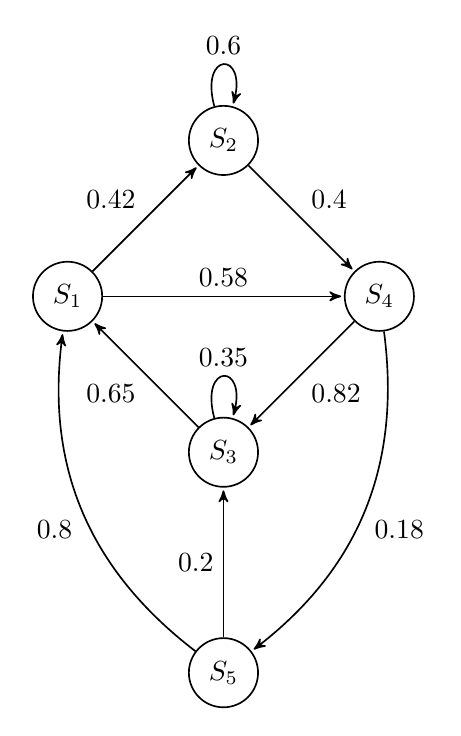
\begin{tikzpicture}[->,>=stealth',shorten >=1pt,auto,node distance=2.8cm,
        semithick,]
    \tikzstyle{every state}=[fill=white,draw=none,text=black,draw=black]
  
    \node[state] (A)                    {$S_1$};
    \node[state]         (B) [above right of=A] {$S_2$};
    \node[state]         (D) [below right of=A] {$S_3$};
    \node[state]         (C) [below right of=B] {$S_4$};
    \node[state]         (E) [below of=D]       {$S_5$};
    
    \path (A) edge              node {0.42} (B)
    edge              node {0.58} (C)
    (B) edge [loop above] node {0.6} (B)
    edge              node {0.4} (C)
    (C) edge              node {0.82} (D)
    edge [bend left]  node {0.18} (E)
    (D) edge [loop above] node {0.35} (D)
    edge              node {0.65} (A)
    (E) edge   node {0.2} (D)
    (E) edge [bend left]  node {0.8} (A);
    \end{tikzpicture}
    \captionof{figure}{Markov chain with state space and transition probabilities}
\end{center}
A Markov Decision Process (MDP) is a generalisation of this framework to sequential
decision making \cite{sutton2018reinforcement}. An MDP consists of an agent-environment
interface, where the \emph{Agent} is the learner and decision maker and the \emph{Environment}
consists of everything outside of the agent. The agent interacts with the environment
bny taking action $a \in \mathbf{A}$ in the current state $S_t$ and receives a reward $R_{t+1}$\footnote{Reward received at $t+1$ to indicate the fact that 
an action must be taken first to move to a new state in order to obtain a reward}, the outcome of the agents actions
transitions the environment from state $S_t$ to $S_{t+1}$.
The agent's long term reward is maximised by taking actions that move the agents into 
favourable states that yield higher rewards, the \textbf{expected} reward in any given state
is equal to the probability of entering state $S_{t+1}$ multiplied by the value of the reward $R_{t+1}$ in that state.
\begin{equation}
    {\displaystyle \E_{S \in \mathbf{S}^n}\biggl[R_{t+1} \; | \; S_t, A_t \biggl] = 
    P(R_{t+1}\; | \; S_t, A_t)\cdot R_{t+1}}
\end{equation}
The \emph{value} of a given state $\mathcal{V}(S)$ is the total expected reward for that state for any action taken in that state.
This is taken to be the \emph{long run} return of state $S$ if the process was repeated in the infinite limit under a stationary distribution of rewards\footnote{
    "Stationary" indicating that the probability of receiving a reward in any state does not change as the process evolves
}:
\begin{equation}
    { \displaystyle \mathcal{V}(S) = \sum_{\forall a \in \mathbf{A}} \E_{S \in \mathbf{S}^n}\biggl[R_{t+1} \; | \; S, a \biggl]}
\end{equation}
An agent in the environment seeks to take actions that maximise its long term reward at each timestep:
\begin{equation}
    \sum_{t \in \mathbf{T}}\underset{a}{max}\biggl(\E_{S \in \mathbf{S}^n}\biggl[R_{t+1} \; | \; S_t, a \biggl]\biggl)
\end{equation}
In episodic settings the set of tasks underlying the MDP contains a \emph{terminal} state that is reached after 
a finite number of timesteps, whereas continuous processes may not necessarily 
have a finite number of time steps. These settings can be unified under the notion of an \emph{absorbing} state $\mathbf{\tau}$
which is one that transitions only to itself with a reward of $R_\tau = 0$.
For a given MDP, successive runs from $S_0$ to $S_\tau$ are termed episodes. In applied settings, an agent
will repeatedly play through episodes with the \emph{Goal} of maximising the cumulative reward in each episode:
\begin{equation}
    G_t \coloneqq R_{t+1} + R_{t+2} + \hdots + R_{\tau-1} = \sum_{t=0}^{t=\tau - 1} R_{t+1}
\end{equation}
Equations (2.15-18) assume a stationary distribution of rewards, and (2.18) is incompatible with continuous domains where
the cumulative reward that the agent tries to maximise can be infinite if $\tau = \infty$. Many real world
tasks such as playing video games \cite{Mnih2015} and dialogue generation \cite{Weisz2018} fall into the category
of continuous, non-stationary MDPs.\\
By instead considering the \emph{discounted cumulative reward}, the analysis of both episodic and continuous 
tasks with non-stationary distributions of rewards becomes computationally tractable:
\begin{equation}
        \begin{gathered}
            0 < \gamma \leqslant 1  \\
            R_{t+1} + \gamma R_{t+2} + \gamma^2 R_{t+3} \hdots + \gamma^{\tau-t-1}R_{\tau-1}
        \end{gathered}
\end{equation}
Where $\gamma$ is referred to as the \emph{discount factor}. The use of a discount
factor contracts rewards further into the future asymptotically towards zero as (2.19) forms a geometric
series\footnote{See Appendix A.3} with ratio $r < 1$:
\begin{equation}
    \begin{gathered}
        \lim_{n \rightarrow \infty} \biggl( \sum_{k= 0}^{n} \alpha \cdot r^k \biggl) = \frac{\alpha}{1-r}, \;\; \forall \; 0 < r < 1, \;\;\; \alpha \in \mathbb{R}^+ \\
    \lim_{n \rightarrow \infty}\biggl(\sum_{k=0}^n 1 \cdot \gamma^k \biggl) = \frac{1}{1 - \gamma}
    \end{gathered}
\end{equation}
Intuitively, this ensures that the agents values immediate rewards more so than delayed rewards as
the rewards in the current timestep can be more accurately estimated than rewards further into 
the future due to the non-stationarity of the process.
And so we can rewrite (2.19) in terms of cumulative reward (2.18):
\begin{equation}
    \begin{gathered}
        G_t = R_{t+1} + \gamma R_{t+2} + \gamma^2 R_{t+3} \hdots + \gamma^{\tau-t-1}R_{\tau-1}\\
        = R_{t+1} + \gamma \biggl[R_{t+2} + \gamma R_{t+3} + \hdots +\gamma^{\tau-t-2}R_{\tau-1} \biggl] \\
        = R_{t+1} + \gamma G_{t+1}
    \end{gathered}
\end{equation}
From (2.22) we can see that a stationary process (2.18) is a special case of the cumulative
discounted reward where $\gamma = 1$. The closer the discount factor is to 1, the more
the agent values future rewards.\\
In order for an agent to choose actions that maximise the discounted future rewards, it 
must adhere to a \emph{policy} $\pi$. A policy is a mapping of states to a distribution
of possible actions:
\begin{equation}
    \begin{gathered}
        \pi: \mathbf{S} \rightarrow P(\mathbf{A}) \\
        \sum_{a \in \mathbf{A}} \pi(a \: | \: s) = 1, \;\;\; \forall s \in \mathbf{S}
    \end{gathered}
\end{equation}
Under this policy, the \emph{value} of a state (2.16) can be rewritten as:\footnote{Needs further derivation}
\begin{equation}
    \begin{gathered}
        \upsilon_\pi(s) = \sum_{a \in \mathbf{A}}\pi(a \: | \:s) \cdot \E \biggl [R_{t+1} + \gamma G_{t+1} \biggl | S_t = s \biggl] \\
        = \E_\pi \biggl [R_{t+1} + \gamma G_{t+1} \biggl | S_t = s \biggl]
    \end{gathered} 
\end{equation}
Equation (2.24) describes an agent's \emph{state-value} function, which measures
the expected return of a given state if the process was repeated infinitely. Similarly,
we can define the \emph{action value} function $q_\pi(s,a)$ to express the average return
of taking a particular action in a given state:
\begin{equation}
    q_\pi(s,a) = \E_\pi \biggl [R_{t+1} + \gamma G_{t+1} \: \biggl | \: S_t = s,\textcolor{red}{ A_t = a} \biggl]
\end{equation}
Formally, the \emph{action value} function describes the expected return of being in state $s$ and taking
action $a$ and following $\pi$ thereafter. It it expected reward described in (2.24) conditioned
additionally upon a fixed action being taken in the current state.
\subsubsection{Bellman Equation}
The state value function and the action value fuction for a given MDP can be estimated from
experience, the Bellman Equation combines the equations described so far and codifys
the relationship between the value of a state and the value of succesor states:
\begin{equation}
    \begin{gathered}
        \upsilon_\pi(s) = \E_\pi \biggl[ R_{t+1} + \gamma G_{t+1}\: \biggl | \: S_t = s  \biggl ] \\
        = \sum_{a \in \mathbf{A}} \pi(a \: | \: s) \sum_{s' \in \mathbf{S}} \sum_{r\in \mathbf{R}}P(s',r \: | \: s,a) \biggl(r + \gamma \E_\pi \biggl [r + G_{t+1} \: \biggl | \: S_{t+1} = s' \biggl] \biggl)\\
        =\sum_{a \in \mathbf{A}} \pi(a \: | \: s) \sum_{s' \in \mathbf{S}} \sum_{r\in \mathbf{R}}P(s',r \: | \: s,a) \biggl(r + \gamma \upsilon_\pi(s') \biggl )
    \end{gathered}
\end{equation}
This represents a weighted sum of the expectations over all possible next states given the current state
$s$ and action taken $a$ \cite{sutton2018reinforcement}.
\subsubsection{Optimality}
Optimal state and value functions ($\upsilon_*, q_*$) are those that maximise the expected return under policy
$\pi$. A policy $\pi$ is defined to be better or equal to policy $\pi '$ if its expected
return is greater or equal to $\pi '$ for all states.\\
\begin{equation}
    \begin{gathered}
        \upsilon_*(s) = \underset{\pi}{max}\: \upsilon_\pi(s) \\
        q_*(s) = \underset{\pi}{max}\: q_\pi(s,a) \\
        \mathlarger{\Rightarrow} \;\; q_*(s) = \E \biggl [ R_{t+1} + \gamma \upsilon_*(S_{t+1}) \: \biggl | \: S_t = s, A_t = a \biggl ]
    \end{gathered}
\end{equation}
As $\upsilon_*$ is the optimal value function, its expected return must equal the expected
return for greedily selecting the \emph{best action} in that state everytime, otherwise there would exist $\upsilon_{\pi*} > \upsilon_*$:
\begin{equation}
    \begin{gathered}
        \upsilon_*(s) = \underset{a \in \mathbf{A}}{max} \; q_{\pi*}(s,a) \\
        = \underset{a}{max} \; \E_{\pi*} \Condition{R_{t+1} + \gamma \upsilon_*(S_{t+1})}{S_t =s, A_t = a}  \\
        = \underset{a}{max} \sum_{s' \in \mathbf{S}} \sum_{r \in \mathbf{R}}P(s',r \:| \:s,a)[r +\gamma \upsilon_*(s')]
    \end{gathered}
    \qquad \text{by (2.27)}
\end{equation}
From (2.28) we can see that the optimal value function is defined independently of any policy, indicating that
it can be reached starting from any arbitary policy, and improving on that, this is formalised under the
framework of \emph{Generalised Policy Iteration} (GPI).
\subsubsection{Generalised Policy Iteration}
GPI consists of an alternating process of making the value function
more accurate with respect to the policy and making the policy
greedy with respect to the current value function. This process
is decomposed into two separate steps:
\begin{enumerate}
    \item \textbf{Policy Evaluation} \\
        An initial value function $\upsilon_0$ is parameterised with arbitary values for each $s \in \mathbf{S}$.
        Given a sequence of value functions $\upsilon_0, \upsilon_1, \upsilon_2, \hdots$ each succesive value
        can be calculated by:
        \begin{equation}
            \upsilon_{k+1}(s) = \E_\pi \Condition{R_{t+1} + \gamma \upsilon_{k}(S_{t+1})}{S_t = s}
        \end{equation}
        The value of each state $s \in \mathbf{S}$ is updated "in place" with the revised estimate garnered
        from the current reward (which may not have been achieved previously) and the expected immediate rewards
        approximated by the previous value function. A pass over all $\mathbf{S}$ produces a new state value function.
    \item \textbf{Policy Iteration} \\
        For a given value function, (2.28) shows that the optimal policy is that which greedily
        selections actions that maximise the expected future returns at each state. It follows that:
        \begin{equation}
            \begin{gathered}
                \pi \in \{\Pi\} \coloneqq \;\; \text{Set of all policies}\\
                \upsilon \in \{\Upsilon\} \coloneqq \;\; \text{Set of all value functions}\\
                q \in \{\mathbf{\mathcal{Q}}\} \coloneqq \;\; \text{Set of all action value functions}\\
            \end{gathered}
        \end{equation}
        \begin{equation}
            \forall \; \pi  \; \exists \; q_*  \mid q_* \geq (q' \neq q_*) \Longleftrightarrow \forall \; \pi  \; \exists \; \upsilon_*  \mid \upsilon_* \geq (\upsilon' \neq \upsilon_*)
        \end{equation}
        \begin{equation}
            \begin{gathered}
                \pi' \geq \pi \; \to \; \upsilon_{\pi'}(s) \geq \upsilon_{\pi}(s) \;\;\;\; \forall s \in \mathbf{S} \\
                \therefore \;\;  q_{*}^{\pi'}(s,a) \geq q_{*}^{\pi}(s,a) \\
            \end{gathered}
        \end{equation}
        \begin{equation}
            \Rightarrow q_\pi(s, \pi'(s)) \geq \upsilon_\pi(s)
        \end{equation}
        This inductive line of logic reasons that if $\exists \; \pi' \geq \pi$ then the expected 
        returns of a given state calculated under policy $\pi'$ will be higher, thus if the less
        optimal policy had instead chosen the action according to the optimal policy, then the expected returns would be
        greater (2.33). The optimal policy is obtained by making the current policy greedy with
        respect to the action value function:
        \begin{equation}
            \begin{gathered}
                \pi'(s) = \underset{a}{argmax} \; q_\pi(s,a) \\
                = \underset{a}{argmax} \sum_{s' \in \mathbf{S}}\sum_{r \in \mathbf{R}}P(s',r \;, | \; s,a) \biggl [r + \upsilon_\pi(s') \biggl]
            \end{gathered}
        \end{equation}
\end{enumerate}

By succesively cycling through policy evaluation and improvement, we 
continuously update our estimate of the value function and then greedily select
actions in each state according to our updated estimates. This cycle is referred to
as \emph{Generalised Policy Iteration} and can be proven to monotonically converge to
an optimal value function and an optimal policy. Upon convergence, the process reaches an
equilibrium where the policy does not change because the value of the states has not changed \cite{sutton2018reinforcement}.
\subsubsection{Exploration vs Exploitation}
The full reinforcement learning problem can be characterised by the models we have described so far
with the addition of the exploration - exploitation trade off. So far we have considered agents with full knowledge of the environment, but
for many MDPs, the agent may never access all available state action pairs, or indeed the number of state action
pairs may be unenumerable. In order to maximise returns, the agent must strike a balance between exploring new, unseen states and exploiting
the greedy strategy it has already learned. A naive exploration strategy\footnote{More recent and general exploration strategies are discussed
in \textbf{2.2.3.2} and \textbf{Related Work}.} is to choose the greedy action with fixed probability
$\mathbf{\varepsilon}$ and otherwise choose a random action with probability $1-\varepsilon$; this is called an
\textbf{$\varepsilon$ greedy strategy}. However the agent would still require an infinite
amountof episodes to form the optimal policy and value functions, they must instead be approximated
in such a way that preserves the gurantees of GPI.
\subsubsection{Monte Carlo Estimation}
Monte carlo estimation enables an agent to \emph{learn} optimal policies and value functions
from experience alone. In order to take advanatge of Monte Carlo methods, the MDP
is modelled in the following way:
\begin{itemize}
    \item Each state has its own stationary distribution of rewards.
    \item Each state is inter-related, i.e taking an action in one state depends on actions taken in later states.
    \item As all action selections are undergoing learning, the distribution of rewards becomes \emph{non-stationary}
    from the point of view of later states. 
\end{itemize}
Monte Carlo methods sample average returns for a given state-action pair for a given
episode and use those samples to update estimates of action values.
Two distinct approaches enable us to do so:
\begin{enumerate}
    \item \textbf{On Policy Methods} \\
        In "\emph{On Policy Control}" we aim to evaluate or improve
        the policy that is used to make decisions, which in turn produces data in the
        form of the outcomes of these decisions.
    \item \textbf{Off Policy Methods} \\
        In "\emph{Off-Policy Control}" attempt to improve a policy different than the
        one used to generate the data.
\end{enumerate}
Within the scope of this project we will focus on \emph{Off Policy} methods.
First we consider two policies $\pi \neq b$ and we refer to the former as the \emph{target}
policy and the latter as the \emph{behaviour} policy. The goal is to estimate $\upsilon_\pi$
or $q_\pi$. We also assume that $\pi(a\:|\:s) > 0 \rightarrow b(a \:|\:s) >0$ implying that 
every action taken under $\pi$ is also taken at least once under $b$; this is the assumption of \emph{coverage}.
From coverage it follows that $b$ must be stochastic in states where it is not identical to
$\pi$ as $\pi_*$, being the optimal policy, is greedy and deterministic.\\
First I will introduce \emph{importance sampling}, a method for estimating
expected values under on distribution given samples from another distribution. This is 
a general technique used in off-policy methods \cite{sutton2018reinforcement} as well as in later discussed \emph{Prioritised
Experience Replay}\footnote{See \textbf{Memory}}. Given a starting
state $S_t$ the probability of a subsequent state action trajectory $A_t, S_{t+1}, A_{t+1}, \hdots $ is :
\begin{equation}
    \begin{gathered}
        \pi \condition{A_t}{S_t} \cdot P\condition{S_{t+1}}{S_t, A_t} \cdot \pi \condition{A_{t+1}}{S_{t+1}} \hdots P\condition{S_T}{S_{T-1}, A_{T-1}} \\
        = \prod_{k=t}^{T-1}\pi\condition{A_k}{S_k} \cdot P\condition{S_{k+1}}{S_k,A_k}
    \end{gathered}
\end{equation}
Therefore, in order to calculate the relative probability (importance samplig ratio) of a trajectory given the
target policy and and the behaviour policy:
\begin{equation}
    \begin{gathered}
        \rho_{t:T-1} = \frac{\prod_{k=t}^{T-1}\pi\condition{A_k}{S_k} \cdot P\condition{S_{k+1}}{S_k,A_k}}{\prod_{k=t}^{T-1}b\condition{A_k}{S_k} \cdot P\condition{S_{k+1}}{S_k,A_k}} \\
        = \prod_{k=t}^{T-1}\frac{\pi\condition{A_k}{S_k}}{b\condition{A_k}{S_k}}
    \end{gathered}
\end{equation}
Intuitively, this is a ratio of how much more or less probably the trajectory is under $\pi$ relative to $b$,
given that $\upsilon_b(s) = \E\Condition{G_t}{S_t = s}$ we can transform
the returns under $b$ to have to correct expected value by multiplying them
by the importance sampling ratio:
\begin{equation}
    \E\Condition{\rho_{t:T-1}G_t}{S_t = s} = \upsilon_\pi(s)
\end{equation}
In the case of full monte carlo methods, the returns are averaged at the end of each episode,
\emph{weighted importance sampling} applies the importance sampling ratio as weighted
average of the returns over the whole episode with terminal state $T(t)$to form our \emph{estimate} $V$:
\begin{equation}
    V_\pi(s) = \frac{\sum_{t \in T(t)} \rho_{t:T-1} \cdot G_t}{\sum_{t \in T(t)} \rho_{t:T-1}}
\end{equation}
This can be rewritten as an incremental update that occurs on an episode by episode basis where
we start with random weights $W_i$ and for each state maintain the cumulative sum of the weights
given to the first $n$ returns ($C_n$):
\begin{equation}
    \begin{gathered}
        W_i = \rho_{t_i : T(t_i) -1}\\
        C_n = \sum_{k = 1}^{n} W_k\\
        V{n+1}(s) = V_{n}(s) + \frac{W_n}{C_n} \biggl [\textcolor{red}{G_n -\upsilon_{n}(s)} \biggl]
    \end{gathered}
\end{equation}
Where the text in red is a \emph{target update} as measurement of the error betweenthe actual returns for that episode $G_n$ and
the previously estimated returns $\upsilon_n(s)$. This is then multiplied proportionally by a
weighted importance sampling ratio. The original estimate of $\upsilon_n(s)$ is the updated
proportionally in the direction towards the actual expected returns.
\subsubsection{Model Free vs Model Based}
Sometimes it is possible to provide the agent with access to a model of the environment.
If an agent has access to a model of the environment, typically in the form of a simulator, it
can simulate states $n$ steps ahead and use that to inform its estimated returns trivially using
the approaches described so far. The trouble with this approach however is that when modelling
a real world task, no coarse grained model will ever approximately the task perfectly. A poorly 
designed model can also introduce unintended biases into the agent \cite{sutton2018reinforcement}.
On the other hand model free methods, such as monte carlo estimation, can approximate the state value or
action value function directly, and have shown better generalization properties with regard
to acting in unforseen scenarios.\\
In this project I will focus on the model-free off-policy methods
as I will show that the PSP problem on a lattice is a non-stationary MDP for which
a model is not computationally tractable. With the foundations lain, I will introduce
the central algorithm to contemporary reinforcement learning.
\subsection{Deep Q Learning}
\subsubsection{Temporal Difference Error}
The temporal difference (TF) error is a special case of monte carlo estimation where the action
value functions and the state value functions are updates with each timestep instead of at the end of each episode.
\begin{equation}
    V(S_t) \leftarrow V(s_t) + \alpha \biggl[\textcolor{red}{R_{t+1} + \gamma V(S_{t+1}) - V(S_t)} \biggl]
\end{equation}
This is similar to the target update in monte carlo estimation, however instead our we update
our existing estimate based on our current estimate, the target in (2.39) is expanded using (2.22).
In this particular case for each episode the agent takes an action, observes the outcome of this action at $S_{t+1}$
and evaluates the value function at this timestep; this evaluation is then used as part of a target update
that is weighted by some constant step size parametere $a$.
\subsubsection{Q Learning}
We can go a step further and unpack (2.40) some more by observing (2.28) and (2.32 - 34) to
form an estimate of our action value function $Q$ directly forming an off policy TD control update rule:
\begin{equation}
    Q(S_t,A_t) \leftarrow Q(S_t,A_t) + \alpha \biggl [R_{t+1} + \gamma \cdot \underset{a}{max} \: Q(S_{t+1}, a) - Q(S_t,A_t) \biggl ]
\end{equation}
This update target is formally known as the \emph{Bellman Error} denoted $\delta_t$. I introduce 
the central algorithm \cite{sutton2018reinforcement}:
\begin{algorithm}[!htb]
    \SetAlgoLined
     $\alpha \in (0,1]$\;
     $0 < \varepsilon < 1$\;
     Init Q(s,a) $\forall \; s \in \mathbf{S}, \: a \in \mathbf{A}(s)$ randomly\;
     Q(terminal, $\cdot$) = 0\;
     \ForAll{episodes}{
      Init S\;
      \ForAll{steps in episode}{
          $r \backsim  U(0,1)$\tcp*[l]{Sample random number r} 
       \eIf{$r > \varepsilon$}{
            $A \leftarrow \underset{a}{argmax}\;Q(s,a)$\;
       }{
            $A \leftarrow rand(a \in \mathbf{A})$ \tcp*[l]{Choose a random action} 
       }
       Take action A, observe R, S' \;
       $Q(S,A) \leftarrow Q(S,A) + \alpha[R +\gamma \cdot \underset{a}{max}Q(S',a) - Q(S,A)]$ \;
       $S \leftarrow S'$
       }
     }
     \caption{Q Learning }
\end{algorithm}
The Q learning algorithm forms the core of methods discussed and proposed throughout this project.
After a brief review of neural networks, I will show how they can parameterise the Q function.
\subsubsection{Neural Networks}
A neural network is a universal non-linear function approximator. It
consists of smaller sub units called perceptrons. Each perceptron acts as linear
function with respect to its inputs $\mathbf{x}$ and can be parameterised by a weight
vector $\mathbf{w}$ and bias $b$.
\begin{equation}
    \mathbf{\hat{y}} =\mathbf{x} \cdot \mathbf{w}^\top + b
\end{equation}
Perceptrons canbe organised into layers hence become multi-layer perceptrons MLP.
If an MLP contains more than a single intermediate layer between the input and the output
layer, it is known as a deep neural net. When organised into layers, the output
of each perceptron must be passed through a non-linearity \[ReLU(\mathbf{\hat{y}}) = max (\mathbf{\hat{y}},0)\] to remove the correlation between
layers, unlocking its potential as a non-linear function approximator.
Contemporary architecture use non-linearities such as rectified linear units (ReLU)
as they demonstrate faster convergence due to sparser representations induced by zeroing weights less than zero.
\begin{center}
    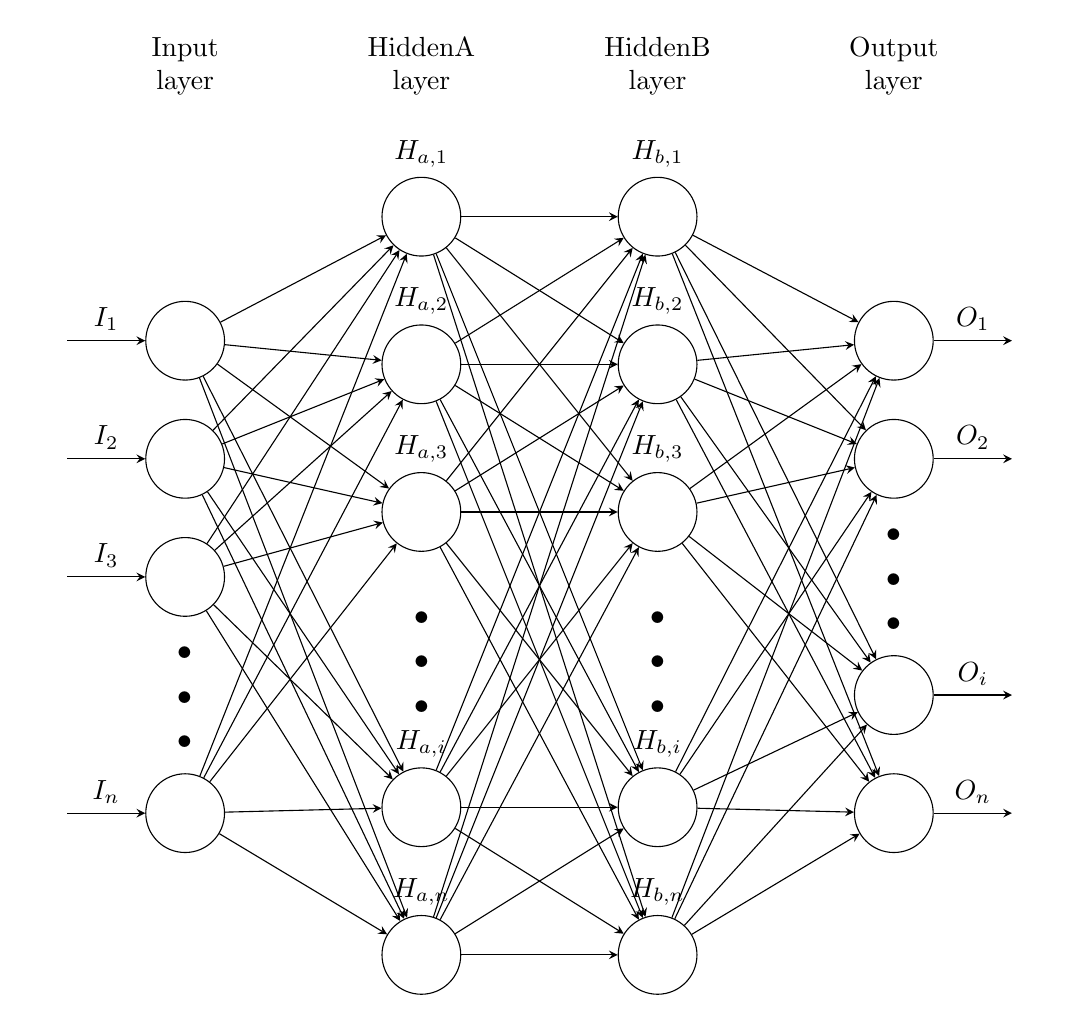
\begin{tikzpicture}[x=1.5cm, y=1.5cm, >=stealth]

    \foreach \m/\l [count=\y] in {1,2,3,missing,4}
      \node [every neuron/.try, neuron \m/.try] (input-\m) at (0,1-\y) {};
    
    \foreach \m [count=\y] in {1,2,3,missing,4,5}
      \node [every neuron/.try, neuron \m/.try ] (hiddenA-\m) at (2,2.3-\y*1.25) {};
    
    \foreach \m [count=\y] in {1,2,3,missing,4,5}
      \node [every neuron/.try, neuron \m/.try ] (hiddenB-\m) at (4,2.3-\y*1.25) {};
      
    \foreach \m [count=\y] in {1,2,missing,3,4}
      \node [every neuron/.try, neuron \m/.try ] (output-\m) at (6,1-\y) {};
    
    \foreach \l [count=\i] in {1,2,3,n}
      \draw [<-] (input-\i) -- ++(-1,0)
        node [above, midway] {$I_\l$};
    
    \foreach \l [count=\i] in {1,2,3,i,n}
      \node [above] at (hiddenA-\i.north) {$H_{a,\l}$};
    
    \foreach \l [count=\i] in {1,2,3,i,n}
      \node [above] at (hiddenB-\i.north) {$H_{b,\l}$};
    
    \foreach \l [count=\i] in {1,2,i,n}
      \draw [->] (output-\i) -- ++(1,0)
        node [above, midway] {$O_\l$};
    
    \foreach \i in {1,...,4}
      \foreach \j in {1,...,5}
        \draw [->] (input-\i) -- (hiddenA-\j);
    
    \foreach \i in {1,...,5}
        \foreach \j in {1,...,5}
            \draw [->] (hiddenA-\i) -- (hiddenB-\j);  

    \foreach \i in {1,...,5}
      \foreach \j in {1,...,4}
        \draw [->] (hiddenB-\i) -- (output-\j);
    
    \foreach \l [count=\x from 0] in {Input, HiddenA, HiddenB,Output}
      \node [align=center, above] at (\x*2,2) {\l \\ layer};
    
    \end{tikzpicture}
\end{center}
A network can be represented as a function $f$ parameterised by weight
matrix $\mathbf{W}$ and bias matrix $\mathbf{b}$ with the outputs of each
layer being passed into the next layer in a fully connected network.
\begin{equation}
    \mathbf{\hat{y}}= f(\mathbf{x}; \mathbf{W}, \mathbf{b})
\end{equation}
The network is optimised against a target output $Y$ using stochastic gradient descent.
\begin{equation}
    \begin{gathered}
        L(Y, \mathbf{\hat{y}}) = \Vert Y - \mathbf{\hat{y}} \Vert_{2} \\
        = \frac{1}{N} \cdot \sum_{i=1}^{N} (Y_i - (\mathbf{x}_i \cdot \mathbf{w}_i^\top + b))^2
    \end{gathered}
\end{equation}
\begin{equation}
    \begin{gathered}
        \frac{\partial E}{\partial \mathbf{w}} = -\frac{2}{N} \cdot \sum_{i=1}^{N} \mathbf{x}_i(Y_i-(\mathbf{x}_i \cdot \mathbf{w}_i^\top +b)) \\
    \frac{\partial E}{\partial b} = -\frac{2}{N} \cdot \sum_{i=1}^{N} (Y_i-(\mathbf{x}_i \cdot \mathbf{w}_i^\top +b))
    \end{gathered}
\end{equation}
\begin{gather}
    \begin{aligned}
        \nabla_{\mathbf{W}} E = \frac{\partial L(Y, \mathbf{\hat{y}}) }{\partial \mathbf{W}}  \,, \;\;\; &
        \nabla_{\mathbf{b}} E = \frac{\partial L(Y, \mathbf{\hat{y}})}{\partial \mathbf{b}} \,
    \end{aligned} 
\end{gather}
The error is calculated first for the network's output layers, the weights are then updated in the direction of 
negative gradient, steepest descent with respect to error $E$ with some constant stepsize $\eta$:
\begin{equation}
    \mathbf{W}_{k+1}=\mathbf{W}_{k} - \eta \nabla E_{\mathbf{W}_k}
\end{equation}
The gradients for the biases are updates likewise. This error is then back-propagated
using reverse mode differentiation on a computational graph \cite{Margossian2019} through the remaining nodes,
where the weights adjusted after the gradient updates are used as the target for the preceeding layer.
\begin{remark}
    In recent years additional properties of neural networks have been discovered
    relating to their nature as universal function approximators. Neural networks with
    a single hidden layer can approximate any function, and as the number
    of nodes tends to infinity it simplifies to a linear model \cite{Jaehoon2019}. Alternatively, infinitely
    wide, deep neural networks are equivalent to a gaussian process \cite{Jaehoon2017}.
    The have also demonstrated the ability to sort lists in practically $O(1)$ time \cite{Xiaoke2019}.
\end{remark}
\subsubsection{Deep Q-Networks}
Neural networks can be used to approximate the Q function directly using Q learning, however the structure
of the gradient update introduces complexity when trying to estimate expected value of rewards. We begin by 
parameterising our Q fuction with the weights of our network:
\begin{equation}
    \begin{gathered}
        Q(s,a)= f(\mathbf{s}; \mathbf{W}, \mathbf{b}) \;\;\;\; s \in \mathbf{S}\\
        \Rightarrow Q(s,a ; \mathbf{W}, \mathbf{b}) \rightarrow Q(s,a ; \mathbf{W}) \\
    \end{gathered}
\end{equation}
We can develop a loss function in the off policy setting using the Bellman Error $\delta_t$.
This holds because the update target $R_{t+1} + \gamma \max_a Q(S_{\textcolor{red}{t+1}},a)$ acts as a
"peek ahead" from the perspective of the current state. That is we take an action, observe the
outcome, and update the action-value of our old state with this new information.
\begin{equation}
    \begin{gathered}
        L(\delta_t, Q(s,a; \mathbf{W})) = \Vert \delta_t - Q(s,a; \mathbf{W}) \Vert_2 \\
        \frac{\partial L(\delta_t, Q(s,a;\mathbf{W} )) }{\partial \mathbf{W} } = \frac{\partial (\delta_t - Q(s,a; \mathbf{W}))^2}{\partial \mathbf{W}}\\
        = (\delta_t - Q(s,a; \mathbf{W})) \cdot \frac{\partial (\delta_t - Q(s,a; \mathbf{W}))}{\partial \mathbf{W}} \\
        = (\delta_t - Q(s,a; \mathbf{W})) \nabla_{\mathbf{W}} Q(s,a; \mathbf{W})
    \end{gathered}
\end{equation}
The target acts as a constant because the maximal estimated Q value at the next state is taken
to be the value of the state under the optimal policy (see 2.32). In their original paper, \cite{Mnih2015}
used a neural network to take in the state as input and then output a vector of action values, 
one for each action. If we used the intepretation of Q learning developed in (2.41), this structure could lead to unstable
gradient updates or could cause the action values to diverge. This can be described
in terms of the correlation between various elements of the model, consider
two dependent random variables $X$ and $Y$:
\begin{equation}
    \begin{gathered}
        Correlation(X,Y) = \frac{Covar(X,Y)}{\sqrt{Var(X)Var(Y)}} \\
        %Correlation(X,Y) \propto Covar(X,Y) \\
        %Correlation(X,Y) \propto \mathbb{E}[(X - \mathbb{E}[X])(Y - \mathbb{E}[Y])] \\
        %\propto \mathbb{E}[XY - X\mathbb{E}[Y] - Y\mathbb{E}[X] + \mathbb{E}[X]\mathbb{E}[Y]] \\
        %\propto \mathbb{E}[XY] - \mathbb{E}[X]\mathbb{E}[Y] - \mathbb{E}[Y]\mathbb{E}[X] + \mathbb{E}[X]\mathbb{E}[Y] \\
        %\propto \mathbb{E}[XY] - \mathbb{E}[X]\mathbb{E}[Y]\\
    \end{gathered}
\end{equation}
The corelation between two dependent random variables is proportional to the covariance of
the random variables normalised by their joint standard deviatiation $\sqrt{Var(X)}= \sigma$.
As correlation is a dimensionless constant on the interval $[-1,1]$, if $X$ and $Y$ are
correlated $Corr(X,Y) \approx 1$, then they increasingly co-vary across each dimension, then their
standard deviation must increase likewise, and as the co-variance goes to infinity, so does their
individual variance. And so under (2.41) we would be using a very similar distribution of
weights to calculate $\max_a Q(S_{t+1}, a)$ and $Q(S_{t}, a)$ which are both dependent 
according to the definition of our MDP. In addition to that, if we consider
successive frames of pixels on a screen as our states, it is trivial note that these
observations will also be highly correlated; in the case of the atari game "Pong", the
position on the paddle on the next frame is highly informed by position of the paddle in the next frame.

Instead, \cite{Mnih2015} propose two solutions to this problem. A biologically
inspired mechanism termed \emph{Experience Replay} and a separate \emph{Target Network}.
To remove the correlations between succesive observations $(S_t,A_t,R_{t+1},S_{t+1})$, they
instead store these tuples in a \emph{replay buffer}. In this case the replay buffer is a FIFO
array of constant size that overwrites older memories with new ones. The target network
is a seperate neural network whose weights $\theta^-$ are initialised with the weights of
the behaviour network and then frozen. Periodically, this target network is updated with the
current weights of the behaviour network $\theta$. 
Every timestep, a batch of memories are uniformly sampled, the target network is used to compute the Bellman Error
for each memory and the output of the behaviour network is updated according to the loss defined in (2.49),
averaged across the whole batch.
This algorithm proceeded to lead a breakthrough in contemporary deep reinforcment learning by outperforming
human benchmarks at a super human level for the first time (adapted from the original authors):
\begin{algorithm}[!htb]
    \SetAlgoLined
    \caption{Deep Q Network (DQN)}
    Init replay memory $D$ to capacity $N$ \;
    Init $Q$ with random weights $\theta$\;
    Init $\hat{Q}$ with $\theta^- = \theta$\;
    \ForAll{episodes}{
        Init state $s_1$\;
        Preprocess sequence $\phi_1 = \phi(s_1)$\;
        \ForAll{timesteps in episode}{
            $r \backsim U(0,1)$\;
            \eIf{r > $\varepsilon$}{
                $a_t \backsim {A}$ \tcp*[l]{ Randomly sample action from action space}
            }{
                $a_t = \underset{a}{argmax}\;\;Q(\phi(s_t),a ; \theta)$\;
            }
            Execute action $a_t$ observe $R_{t+1}, s_{t+1}, d$ \tcp*[l]{$d = 1$ if state is terminal else $0$} 
            Store $(\phi_1,a_t,r_{t+1},\phi_{t+1})$ in $D$\;
            Sampled random minibacth from $D$\;
            $\delta_t = r_t + (1-d) \gamma \max_{a'} \hat{Q}(\phi_{t+1},a'; \theta^-)$\;
            Perform gradient update $(\delta_t - Q(s,a; \theta)) \nabla_{\theta} Q(s,a; \theta)$\;
            Every $C$ steps reset $\hat{Q} = Q$\;
        }
    }
\end{algorithm}

\subsection{Improvements to Vanilla Deep Q-Networks}
Although the initial algorithm was very successful, it came with various stability 
issues arising from different sources. In particular, bootstraped values can be inherently
unstable \cite{sutton2018reinforcement} due to the nature of trying to estimate a guess from
a guess. Additionaly, sampling memories uniformly at random implicitly samples
are larger number of unsuccesful memories (i.e ones that did not attain a reward) than successful
memories as the action selections are initially random and uninformed at the start of training.
The na\"{i}ve $\varepsilon$ greedy policy is also prohibitive; it monotonic decrease across
the training run indicates that the exploration coefficient decreases for all states uniformly.
Another way of stating this is that no matter what state the agent is in, the likelihood
of choosing a random action to explore more of the state space decreases over time.
This may not be a desireable attribute, as we may want to explore more in some states over others,
and this preference for exploration may change over time as learn new information and update
our estimates (via bootstrapping). \\
In follow up work \cite{Hessel2017} combine subsequent improvements to the original DQN algorithm
addressing the issues listed above into a single agent termedthe "Rainbow" agent. I will
go over each of the suggested improvements.
\subsubsection{Prioritised Experience Replay}
The motivation behind \emph{Prioritised Experience Replay} \cite{Schaul2015} is the notion that given
a batch of pre-recorded memories, the agent should ideally prioritise learning 
from certain experiences over others. Their work follows from neuroscientific studies
suggesting that the sequences of memories selected for experience replay in animals
are chosen proportionally to the rewards associated with that sequence and the magnitude of the
$\delta_t$ error. The magnitude of the $\delta_t$ error can be interpreted as the amount of "surprise"
associated with the that sequence, if our estimated Q value for a state action pair was far
from our target, the the result of our actions will always deviate from expectations because we did not
form a reliable way to ascertain the outcome of events. Updating our estimates for events in which
we were surprised is a necessary part of the learning cycle, and so prioritising memories according
to this surprise is warrented.\\
The authors assign a probability of being played to each memory as such:
\begin{equation}
    \begin{gathered}
        p_i = \vert \delta_i \vert + \epsilon \\
        P(i) = \biggl(\frac{p_i}{\sum_k p_k}\biggl)^\alpha
    \end{gathered}
\end{equation}
Where $\epsilon$ is some small positive constant to prevent the priority $p_i$ from being zero
and $P(i)$ is the probability of the transition being chosen for replay. The exponent $\alpha$
determines the amound of prioritisation used where $\alpha = 0$ is uniform (regular experience replay).
However the use of such a distribution introduces bias into the updates of the $Q$ value. The estimation
of an expected value with stochastic updates relies on those updates come from the same distribution as
our estimatiom, by construction the distribution as in (2.51), we are now drawing on observations
from a different distribution than the one underlying the MDP. This is corrected for with 
importance sampling weights introduced in \textbf{2.2.1.5}.
\begin{equation}
    \begin{gathered}
        w_i = \biggl(\frac{1}{N}\cdot \frac{1}{P(i)} \biggl)^\beta \\
        \nabla_\theta E = w_j \delta_j \nabla_\theta Q(S_{j-1}, A_{j-1}\:; \: \theta)
    \end{gathered}
\end{equation}
The bias is fully compensated for at $\beta = 1$ this ofcourse is coupled with a significant
increase in variance. In practice, the authors additionaly normalise the weights with $\frac{1}{\max_i w_i}$
so that the updates only scale downwards to reduce the overall magnitudes of the gradient updates
and $\beta$ is initialised to a low value $\backsim 0.4$ which is 
linearly annealed up to 1, this encourages additional stability during the training procedure.
The observations themselves are stored in a binary heap, specifically a \emph{Sum Segement Tree} rather
than a typical array or buffer:
\tikzset{
  treenode/.style = {align=center, inner sep=0pt, text centered,
    font=\sffamily},
  arn_n/.style = {treenode, circle, black, draw=black,
    text width=2em},% arbre rouge noir, noeud noir
  arn_r/.style = {treenode, circle, black, draw=black,
  text width=2em},% arbre rouge noir, noeud rouge
  arn_x/.style = {treenode, rectangle, draw=black,
    minimum width=0.5em, minimum height=0.5em}% arbre rouge noir, nil
}
\begin{figure}[!htb]
    \caption{Sum Segment Tree}
    \begin{center}
        \begin{tikzpicture}[->,>=stealth',level/.style={sibling distance = 5cm/#1,
            level distance = 1.5cm}] 
            
            \node [arn_n] {1}
            child{ node [arn_r] {0.33}
                        child{ node [arn_n] {0.15} 
                        }
                        child{ node [arn_n] {0.18}
                        }
                    }
                child{ node [arn_r] {0.67} 
                        child{ node [arn_n] {0.25} edge from parent node[above left]
                        {$0.67 - 0.42$} 
                        }
                        child{ node [arn_n] {0.42}
                        }  
                        edge from parent node[above right]
                        {$1 - 0.33$}                           
                }
                
            ; 
            \end{tikzpicture}
    \end{center}
\end{figure}
This offers the added benefit of $O(1)$ max priority read, the root of the tree, and 
$O(log N)$ time to update the priorities of each transition which resides on the leaves of
the tree. To traverse the tree for a batch size of $k$ memories, the interval $[0, p_{total}]$ is divided into $k$ equal intervals.
Each of these intervals is then uniformly sampled to produce a priority in that interval. The
transition whose value is the closest to each sampled priority is then chosen for replay by succesively
subtracting results until you arrive at a leaf as least as big as the query. Using this binary heap structure eliminates the
need for sorting, enabling the speed up in time complexity.
\subsubsection{Dueling Networks}
\cite{Ziyu2015} observed that the action value function can be decomposed
further into a value and advantage function:
\begin{equation}
    Q(s,a) = V(s) + A(s,a)
\end{equation}
Where the advantage is a measure of the advantage of taking an action in that state relative
to other possible actions. The expected value of a state is an estimate that takes into account
all possible action values of that state. Given than some values will be more valuable than others,
the expected value of a state can be taken to represent the weighted mean of all action values. Therefore
the maximal value of the optimal action of a state, will be greater than the mean, this difference is 
expressed as the advantage of that action. Ofcourse, in an optimal setting:
\begin{equation}
    \begin{gathered}
        A(s,a) = 0 \Longleftrightarrow V^*(s) = \max_a Q^*(s,a)\\
        \rightarrow A(s,a) = Q^*(s,a) - V^*(s) = 0
    \end{gathered}
\end{equation}
As the value of a state is the value of the most optimal action, the relative advantage of
the action to itself is $0$. Given only a $Q$ function we cannot recover the value
and advantage and value uniquely due to the nature of the inter-connectedness of the neural
network. Changes in the weights affect the entire space of approximation. Instead
the authors decompose the output layer of the DQN into two seperate heads, one that calculates
the advantage and another to calculate the value (as a scalar).

\definecolor{olivegreen}{rgb}{0,0.6,0}
\begin{figure}[!htb]
    \caption{Dueling Network Heads}
    \begin{center}
        \begin{tikzpicture}

            \path[rounded corners, fill=blue, fill opacity=0.2] (-0.4, 3.5) --  (-0.4, -3.5) -- (4, -3.5) -- (4, -0.2) -- (5, -0.2) -- (5, 3.5) -- (-0.4, 3.5) -- (-0.4, 0);
            \path[rounded corners, fill=red, fill opacity=0.2] (-0.4, -3.5) --  (-0.4, 3.5) -- (4, 3.5) -- (4, -0.2) -- (5, -0.2) -- (5, -3.5) -- (-0.4, -3.5) -- (-0.4, 0);
            \path[rounded corners, fill=white] (-0.4, 0) -- (-0.4, -3.5) -- (4, -3.5) -- (4, 3.5) -- (-0.4, 3.5) -- (-0.4, 0);
            \path[rounded corners, fill=olivegreen, fill opacity=0.2] (-0.4, 0) -- (-0.4, -3.5) -- (4, -3.5) -- (4, 3.5) -- (-0.4, 3.5) -- (-0.4, 0);
            \path [draw, dashed, very thick, rectangle, rounded corners] (-0.4, 0) -- (-0.4, -3.5) -- (5, -3.5) -- (5, 3.5) -- (-0.4, 3.5) -- (-0.4, 0);
            
            \node[circle, thick, fill=white, draw] (x1) {};
            \node[circle, thick, draw, fill=white, below=1em of x1] (x2) {};
            \node[circle, thick, fill=white, draw, below=1em of x2] (x3) {};
            \node[circle, thick, fill=white, draw, below=1em of x3] (x4) {};
            \node[circle, thick, fill=white, draw, below=1em of x4] (x5) {};
            \node[circle, thick, fill=white, draw, above=1em of x1] (x6) {};
            \node[circle, thick, fill=white, draw, above=1em of x6] (x7) {};
            \node[circle, thick, fill=white, draw, above=1em of x7] (x8) {};
            \node[circle, thick, fill=white, draw, above=1em of x8] (x9) {};
            \node[circle, thick, right=4em of x1, fill=white, draw] (xhh1) {};
            \node[circle, thick, draw, fill=white, below=1em of xhh1] (xhh2) {};
            \node[circle, thick, fill=white, draw, below=1em of xhh2] (xhh3) {};
            \node[circle, thick, fill=white, draw, below=1em of xhh3] (xhh4) {};
            \node[circle, thick, fill=white, draw, above=1em of xhh1] (xhh5) {};
            \node[circle, thick, fill=white, draw, above=1em of xhh5] (xhh6) {};
            \node[circle, thick, fill=white, draw, above=1em of xhh6] (xhh7) {};
            \node[circle, thick, right=8em of x1, fill=white, draw] (xh1) {};
            \node[circle, thick, draw, fill=white, below=1em of xh1] (xh2) {};
            \node[circle, thick, fill=white, draw, below=1em of xh2] (xh3) {};
            \node[circle, thick, fill=white, draw, below=1em of xh3] (xh4) {};
            \node[circle, thick, fill=white, draw, above=1em of xh1] (xh5) {};
            \node[circle, thick, fill=white, draw, above=1em of xh5] (xh6) {};
            \node[circle, thick, fill=white, draw, above=1em of xh6] (xh7) {};
            \node[circle, very thick, fill=blue!30, draw, right=12em of x1, yshift=5em] (hm1) {};
            \node[circle, very thick, draw, fill=blue!30, below=0.5em of hm1] (hm2) {};
            \node[circle, very thick, draw, fill=blue!30, below=0.5em of hm2] (hm3) {};
            \node[circle, very thick, draw, fill=blue!30, above=0.5em of hm1] (hm4) {};
            \node[circle, very thick, draw, fill=blue!30, above=0.5em of hm4] (hm5) {};
            \node[circle, very thick, fill=red!30, draw, right=12em of x1, yshift=-5em] (hs1) {};
            \node[right=1.5em of hm1, blue] (mu1) {$A_{\theta_1}(s, \alpha_3)$};
            \node[right=1.5em of hm2, blue] (mu2) {$A_{\theta_1}(s, \alpha_4)$};
            \node[right=1.5em of hm3, blue] (mu3) {$A_{\theta_1}(s, \alpha_5)$};
            \node[right=1.5em of hm4, blue] (mu4) {$A_{\theta_1}(s, \alpha_2)$};
            \node[right=1.5em of hm5, blue] (mu5) {$A_{\theta_1}(s, \alpha_1)$};
            \node[right=1.5em of hs1, red] (s1) {$V_{\theta_2}(s)$};
                
            \foreach \x in {1,...,9}
                \foreach \y in {1,...,7}
                    \draw[-stealth, thick] (x\x) -- (xhh\y);
            
            \foreach \x in {1,...,7}
                \foreach \y in {1,...,7}
                    \draw[-stealth, thick] (xhh\x) -- (xh\y);
            
            \foreach \x in {1,...,7}
                \foreach \y in {1,...,5}
                    \draw[-stealth, thick, blue] (xh\x) -- (hm\y);
            
            \foreach \x in {1,...,7}
                \draw[-stealth, thick, red] (xh\x) -- (hs1);
            
            \draw[-stealth, decoration={snake, pre length=0.01mm, segment length=2mm, amplitude=0.3mm, post length=1.5mm}, decorate, thick, red] (hs1) -- (s1);
            
            \foreach \x in {1,...,5}
                \draw[-stealth, decoration={snake, pre length=0.01mm, segment length=2mm, amplitude=0.3mm, post length=1.5mm}, decorate, thick, blue] (hm\x) -- (mu\x);
                        
            \node[left=0.75em of x1] (l1) {$s$};
        \end{tikzpicture}
    \end{center}
    \scriptsize{\dag Source: \url{https://github.com/PetarV-/TikZ/blob/master/A3C\%20neural\%20network/a3c_neural_network.tex} }
\end{figure}
The action value is then calculated:
\begin{equation}
    Q(s,a \: ; \: \theta) = V(s\:;\:\theta_2 ) + (A(s,a\:;\:\theta_1) - \mathbb{E}[A(s,a\:;\:\theta_1)])
\end{equation}
We fix this lack of identifiability by forcing the function approximator to maximise the
value of the state by having a 0 advantage at the chosen action, hence we subtract the mean.
The $Q$ values for bothe the behaviour and target network are calculated this way.
\subsubsection{Double Q Learning }
Consider the MDP given by fig (2.10),
\begin{figure}[!htb]
    \caption{Maximization Bias Example}
    \begin{center}
        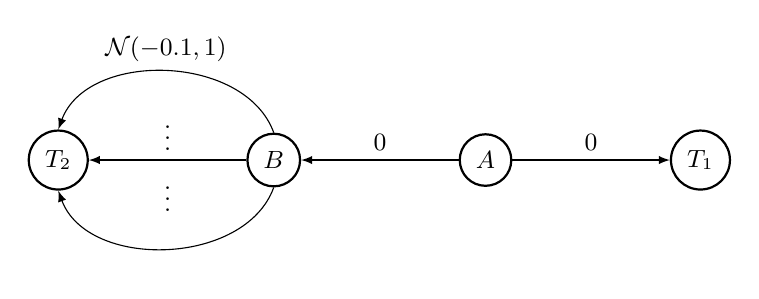
\begin{tikzpicture}[auto,node distance=8mm,>=latex,font=\small]

            \tikzstyle{round}=[thick,draw=black,circle]
        
            \node[round] (s0) {$A$};
            \node[round, right=0mm and 20mm of s0] (s1) {$T_1$};
            \node[round, left=0mm and 20mm of s0] (s2) {$B$};
            \node[round, left=0mm and 20mm of s2] (s3) {$T_2$};
            \draw[->]  (s0) -- (s1) node [midway, above]{$0$};
            \draw[->] (s0) -- (s2) node [midway, above]{$0$};
            \draw[->] (s2.north) to [out=110,in=70] node[above]{$\mathcal{N}(-0.1,1)$} (s3.north);
            \draw[->] (s2) -- (s3) node [midway, above]{$\vdots$} node [midway, below]{$\vdots$};
            \draw[->] (s2.south) to [out=-110,in=-70] node[below]{} (s3.south);
        \end{tikzpicture}
    \end{center}
    \scriptsize{\dag Source: \cite{sutton2018reinforcement}}
\end{figure}
the agent begins in state A and can either move left or right for a reward in 0.
Moving right will terminate the process with reward 0. Moving left (with reward 0)
puts the agent in a state where it can choose amongst a multitude of actions whose
rewards are normaly distributed with a mean of 0.1 and variance of 1.
During policy iteration we select actions according to $\underset{a}{argmax} \: Q(s,a)$,
this incurs a significant \emph{positive} bias due to the nature of the maximization, in
fig (2.10) the agent will always choose the left action as it seeks to maximise the expected
return and certain returns from going to $B$ will be greater than 0; instead the agent should
choose to go right, because the expected value of that action is greater
than the expected value of going to $B \backsim -0.1$.
The error occurs because the same samples are used to determine both the value of each action and to select
the maximising action. \cite{Hasselt2015} address this within the context of deep Q learning
by proposing the following variant of the temporal difference $\delta_t$ error:
\begin{equation}
    y_i = R_{t+1} + \gamma Q(S_{t+1}, \underset{a}{argmax} \: Q(S_{t+1}, A_{t+1}\:;\:\theta)\:;\: \theta^-)
\end{equation}
The Q value of the next state is calculated first by finding the most optimal action for
that next state according to our behaviour policy parameters $\theta$ and then selecting
the Q value of the action according to its value under the target network's parameters $\theta^-$.
By doing so we decouple the estimation of an actions value from its selection. The authors
show that this is effective in combination with the previously discussed improvements.
\subsubsection{Distributional Reinforcement Learning}
Recalling equation (2.41), the expected future discounted reward is a weighted mean,
whose final output is a scalar value. This mean ignors the variance and possible multi-modality
of the underlying distribution. Assuming that the process of generalized policy iteration
reaches a fixed point $\pi^* = \pi_\theta$ where the policy under the neural network's parameters
aproximates the optimal policy arbitarily well, this approximation is only in their means, and equality
of means does gurantee that the "shape" of the underlying distributions are the same.
Motivated by these shortcomings, \cite{Bellemare2017} proposed an alternative distributional perspective
on reinforcement learning. The authors reinterpret equation (2.41) under a distributional variant;
first they contextualize the Q learning update under the \emph{Bellman operator} $\mathcal{T}^\pi$ and in the control setting
as the application of the \emph{"optimality operator"} $\mathcal{T}$:
\begin{equation}
    \begin{gathered}
        x \in \mathbf{S}, \;\; x' \coloneqq x_{t+1}\\
        \mathcal{T}^\pi Q(x,a) = \mathbb{E}[R(x,a)] + \gamma \underset{P,\pi}{\mathbb{E}} [Q(x',a')] \\
        \rightarrow \mathcal{T} Q(x,a) = \mathbb{E}[R(x,a)] + \gamma \underset{P,\pi}{\mathbb{E}} [\max_{a' \in A}Q(x',a')]
    \end{gathered}
\end{equation}
This reflects the same objective as (2.41), where successive applications of the Bellman operator
produce new policies paramterised by the updated estimates to the Q value function. Additionally we recognise
that the reward $R(x,a)$ the agent receives depends on the action taken in that particular state. Under the
distributional setting the state is denoted $x' \backsim P( \cdot \mid x, a)$ as the state is assumed
to be sampled from the underlying steady state distribution of the MDP\footnote{See equation (2.41)}.
Considering the markov property\footnote{See \textbf{2.2.1}}, the discounted future returns $\gamma G_{t+1}$ of a particular state
can be considered a random variable $Z$ distrbuted according to the probability of attaining
certain returns dependent on the action taken in each state, formally $R \in \mathbf{Z}$, where
$\mathbf{Z}$ represents a mapping from state-action pairs to \emph{distributions} of returns.
Furthermore the authors describe "transition operator" as an operator that transforms the current
distribution of discounted returns into the distribution of discounted returns for the next state:
\begin{equation}
    \begin{gathered}
        \mathcal{P}^\pi : Z \mapsto Z'\\
        \mathcal{P}^\pi Z(x,a) \distributed Z(x',a') \\
        x' \backsim P(\cdot \mid x,a), \;\; a' \backsim \pi(\cdot \mid x')
    \end{gathered}
\end{equation}
In this case, the transition operator will map the distribution
of returns under the current state and action, to the distribution returns under the next state action  pair which
is distributed according to the same law (denoted by $\distributed$) as the previous distribution. They then
reformulate the Bellman operator:
\begin{equation}
    \begin{gathered}
        \mathcal{T}^\pi Z(x,a) \distributed R(x,a) + \gamma \mathcal{P}^\pi Z(x,a)
    \end{gathered}
\end{equation}
Three sources of randomness arise under this interpretation:
\begin{itemize}
    \item Randomness in reward $R(x,a)$.
    \item Randomness in the transition $\mathcal{P}^\pi$.
    \item Randomness in the next state-value distribution $Z(x',a')$.
\end{itemize}
These sources are important to observe when considering if the distributional variant of the Bellman equation
converges to a fixed point $Z^\pi$. In order to measure the relative distance between an arbitary distribution,
the authors utilise the \emph{Wasserstein} distance defined on cumulative density functions (c.d.f) of arbitary probability
density functions (p.d.f). If a random variable is distributed according to $F(x)$ then it's c.d.f, also known
as a quantile function, is $F^{-1}(x)$. The \emph{Wasserstein} distance is an $L_p$ metric for some $p \in \mathbb{N}$ that measures the distance
between two random variables $U, V$ on the space of possible samples (values the variable can take on) $\omega \in \Omega$
is the smallest possible difference between the probability density of each sample whose support is the metric space $[0,1]$:
\begin{equation}
    \begin{gathered}
        W_p(F,G) = \biggl ( \int_{0}^{1} \vert F^{-1}_U(\omega) - F^{-1}_{V}(\omega) \vert^p \,\mathrm{d}x \biggl )^{\frac{1}{p}} \\
        = \inf_{U,V} \Vert U - V \Vert_p
    \end{gathered}
\end{equation}
To measure the distance between value distributions $Z_1, Z_2$, they define the maximal form of the Wasserstein metric
as the highest element-wise absolute difference between the two:
\begin{equation}
    \bar{d}_p(Z_1, Z_2) \coloneqq \sup_{x,a} W_p(Z_1(x,a), Z_2(x,a)) 
\end{equation}
The authors show that similarly to equation (2.20) the $\bar{d}_p$ metric is a contraction in $\gamma$
by \emph{Banach's fixed point theorem}\footnote{See Appendix}:
\begin{equation}
    \begin{gathered}
        \bar{d}_p( \mathcal{T}^\pi Z_1, \mathcal{T}^\pi Z_2) \leqslant \bar{d}_p(R + \gamma \mathcal{P}^\pi Z_1, R + \gamma \mathcal{P}^\pi Z_2) \\
        \leqslant \bar{d}_p(\gamma \mathcal{P}^\pi Z_1, \gamma \mathcal{P}^\pi Z_2) \\
        \leqslant \vert \gamma \vert \bar{d}_p(\mathcal{P}^\pi Z_1, \mathcal{P}^\pi Z_2) \\
        \leqslant \gamma \bar{d}_p(Z_1, Z_2) 
    \end{gathered}
\end{equation}
In theory, these results can be applied directly by substituting (2.56) for the Q learning update, however
the issue arises when incorporating function approximation in an effort to parameterise the distribution
of returns for each state-action pair. Starting from random, the network's parameters 
are continually updated to more closely reflect the actual distribution of returns for each state action pair.
As a result, the support\footnote{Range of values that the expected discounted return of a state action pair can take on with a non-zero probability}
of the predicted distribution, the output of the neural network, will drift over time. Generalised policy iteration
continuously produces new policies, in this case, the result is that each policy is defined on a different support.
This poses an issue, as the distance between two random variables on disjoint supports is infinite \cite{Bellemare2017}.
In practice the authors overcome this by utilising a $\mathbf{\Phi}_2$ projection of the output distribution of the network 
onto a discrete support with $N$ atoms and then minimzing the \emph{Kullback Liebler} divergence between the target and the prediction.\\

However as \cite{Dabney2017} note in their follow up work, the conjugation of the $\mathbf{\Phi}_2$ operator with the Bellman operator $\mathcal{T}^\pi$
does not necessarily converge to the \emph{same fixed point} as the repeated application of the $\mathcal{T}^\pi$. Additionally, in practice
the $\mathbf{\Phi}_2$ projection requires conducting a nearest neighbour search between the atoms of the predicted distribution
and the target distribution, and assigning credit proportionally to the 2 nearest neighbours, this can be unwieldy to implement.
\cite{Dabney2017} instead propose \emph{quantile regression} as a way around these limitations.\\

Where \cite{Bellemare2017} choose to fix the support and vary the probabilities,\cite{Dabney2017} invert
this formulation to instead fix the probabilities and vary the support. The complete metric space of
probability $[0,1]$ is discretized into $\tau$ uniform intervals and the appropriate density of returns 
is allocated to each interval. First they show that the projection $\Pi_{W_1}$ of any arbitary value distribution
$Z$ onto a distribution of $\tau$ number of quantiles $Z_Q$, preserves the convergence to a fixed point under the conjugation
of $\bar{d}_p \circ \Pi_{W_1}$:
\begin{equation}
    \bar{d}_p(\Pi_{W_1} \mathcal{T}^\pi Z_1,\Pi_{W_1} \mathcal{T}^\pi Z_2) \leqslant \gamma \bar{d}_p(Z_1, Z_2)
\end{equation}
The Q network aims to predict the quantiles $\theta_i$ for each action  resulting in a vector $Z_\theta \in Z_Q$
for each action such that $Z_{\theta_i} = P(y_i < \theta_i)$\footnote{For instance if $\tau = 6$ then $Z_{\theta_5} = y_i$ s.t $P(y_i < Q(\frac{5}{6})) \mid  F^{-1}(Q(\frac{5}{6})) = \frac{5}{6}$}. 
In order to project an arbitary distribution onto a distribution of $N$ quantiles
it follows that the most suitable distribution is that which minizes the \emph{Wasserstein} metric $\Pi_{W_1}Z= \arg \min W_p(Z, Z_Q)$. 
The authors show that the value on the interval of each quantile that minimizes this distance is the
median of the interval:
\begin{equation}
    \begin{gathered}
        \arg \min \int^{\tau'}_\tau \vert F^{-1}(\omega) - \theta \vert \, d\omega \\
        \text{Is given by} \\
        \theta : F(\theta) = \frac{\tau + \tau'}{2}
    \end{gathered}
\end{equation}
They utilise \emph{quantile regression loss} developed within economics, to fit the predicted
quantile distribution of action-values to a target quantile distribution. Formally, a dirac delta
function positioned on the quantiled is scaled proportionally when the distance $\xi = \hat{Z} - \theta$ 
is overestimated $\xi \geq 0$ or underestimated $\xi < 0$. Quantile regression is used
to fit the predicted quantile to the target by minimizing the following objective:
\begin{equation}
    \begin{gathered}
        \rho_\tau(u) = \begin{cases}
            \tau \cdot u & u \geq 0 \\ %Update this!
            (1 - \tau) \cdot u & u < 0
        \end{cases} \\
        \mathcal{L}^\tau_{QR} \coloneqq  \sum_{i=1}^N \E_{\hat{Z} \backsim Z}[\rho_\tau(\hat{Z} -\theta_i)]
    \end{gathered}
\end{equation}
This is in turn applied to the Bellman update: 
\begin{equation}
    \begin{gathered}
        \mathcal{T}Q(x,a) = \mathbb{E}[R(x,a)] + \gamma \mathbb{E}_{z' \backsim P}[\max_{a'}Q(x',a')] \\
        \rightarrow \mathcal{T}Z(x,a) = R(x,a) + \gamma Z(x',a') \\
        x' \backsim P(\cdot \mid x,a), a' = \arg \max_{a'} \mathbb{E}_{z \backsim Z(x',a')}[z] \\
    \end{gathered}
\end{equation}
From which the authors derive the TD control update:
\begin{equation}
    \theta_i(x) \leftarrow \theta_i(x) + \alpha(\hat{\tau}_i - \delta_{r + \gamma < \theta_i(x)})
\end{equation}
\cite{Dabney2017} results show that learners that incorporate the distribution of returns (\textbf{risk-sensitive learners})
perform much better and converge to optimal policies much faster, this increase in performance is no doubt
due to the greater representational power of distributions.
\section{Multi-Agent Reinforcement Learning}
\subsection{Stochastic Games}
\subsubsection{Game Theory}
\subsubsection{Expected Pay-offs as Expected Rewards}
\subsubsection{Multi-Agent Games}
\subsubsection{Mean Field Games}
\subsubsection{Mean Field multi-agent reinforcement learning}
\section{Related Work}
In this section I will explore and contrast current computational approaches to the PSP problem,
including those that operate over lattices (on-lattice) and relevant techniques and results from
off-lattice prediction methods.
\subsection{MCMC \& Integer Programming methods for lattice models}
Markov Chain Monte-Carlo (MCMC) is a random sampling technique that aims to parameterise
an approximation of the posterior distribution of a given dataset. Data points are sequentially sampled from the target distribution
using arbitary parameters $\theta_1 , \theta_2, \hdots, \theta_n$, the distribution is then approximated
using gradient descent (or hill-climbing) by comparing the ratios of the likelihoods of the posterior 
for each succesive pairs of parameters $\frac{p(data | \theta_2)}{p(data | \theta_1)}$. The parameters of the approximating
distribution are then updated using this ratio, often in addition to a standard learning 
rate $\eta$; this is effectively an optimization in parameter space. The metropolis-random walk algorithm
updates the parameters based on an acceptance criterion. Canonically, a random number is uniformly sampled
on the interval $[0,1]$ and the parameter update is "accepted" if the ratio is greater than the random number.
The sequential sampling produces auto-correlated samples, indicating that each data-point sampled is
probabilistically dependent on the previous point as a function of time; this gives rise to the \emph{markov property}
of the sampling technique. Under this construction, the steady state (equilibrium) distribution of the chain\footnote{See equation 2.14}
is equal to the posterior under investigation; a more thorough analysis is out of the scope of this project however
the reader is directed to \cite{levin2017markov}. \\

\cite{Hansmann1999} gives a detailed overview of markov chain monte-carlo (MCMC) methods and genetic
algorithms for structure prediction. Previous approaches to structure prediction generally involved stochastic
approximation methods such as MCMC in order to tackle the curse of dimensionality when working
with atomic parameters. This often included the use of genetic algorithms
to generate candidate structures and crystal growth simulations where MCMC to randomly
place a residue (obeying SAW constraints) in unrestricted 3D space followed by local optimization
on the structure. In addition to this, if parameter updates are accepted according to a \emph{Boltzmann}
weighting, simulated logarithmic annealing schedules were used to modulate the temperature parameter, often improving results. 
The author notes that although this was effective in smaller peptides, the approaches generally
did not scale to larger structures. Furthermore, the resultant structures would often lack detailed balance;
although the global structure was approximately optimal, residues in local structures would form unfavourable
contacts. \\

\cite{Citrolo2013} describe a hybrid approach between previously mentioned MCMC methods and ant colony optimization (ACO)
using the HP model on a 3D cubic lattice (see eq. 2.7).
ACO is a biologically inspired heuristic search algorithm where each "ant" represents a possible solution, these
agents communicate locally to coordinate their next move towards a more optimal position in parameter space.
The authors present a modified version of the objective function described in table 2.2 that penalizes
overlapping walks. As in previous work, they utilise MCMC to refine a global objective function, and then
use the ants to optimize local solutions. The communication bias between the agents appeared to encourage
better results as compared with previous methods. Once again, this proved to be effective on smaller peptides
but scaling would still be an issue. An insightful observation by the authors suggested that the existence of overlapping
solutions resulted in a rough fitness lanscape, reducing stability during the training phase. \\

\cite{Yanev2017} similarly proposed a mixed integer programming solution to the HP model, once again
on a 3D cubic lattice. Mixed integer programming (MIP) is an optimization method that optimizes constraints
whose requirements are represented by linear relationships, in this particular case some of the constraints
are expressed as integers whereas others may take on real values. The authors evaluate PSP as a bi-partite
graph matching problem on local neighbourhoods, taking into account the SAW. A bi-partite graph in one whose
vertices can be divided into two disjoint and independent sets \cite{Handa1999BipartitieGW}, an example is
provided:

\definecolor{myblue}{RGB}{80,80,160}
\definecolor{mygreen}{RGB}{80,160,80}
\begin{figure}[!htb]
\begin{center}
    \begin{tikzpicture}[thick,
        every node/.style={draw,circle},
        fsnode/.style={fill=myblue},
        ssnode/.style={fill=mygreen},
        every fit/.style={ellipse,draw,inner sep=-2pt,text width=2cm},
        ->,shorten >= 3pt,shorten <= 3pt
      ]
      
      % the vertices of U
      \begin{scope}[start chain=going below,node distance=7mm]
      \foreach \i in {1,2,...,5}
        \node[fsnode,on chain] (f\i) [label=left: \i] {};
      \end{scope}
      
      % the vertices of V
      \begin{scope}[xshift=4cm,yshift=-0.5cm,start chain=going below,node distance=7mm]
      \foreach \i in {6,7,...,9}
        \node[ssnode,on chain] (s\i) [label=right: \i] {};
      \end{scope}
      
      % the set U
      \node [myblue,fit=(f1) (f5),label=above:$U$] {};
      % the set V
      \node [mygreen,fit=(s6) (s9),label=above:$V$] {};
      
      % the edges
      \draw (f1) -- (s6);
      \draw (s6) -- (f2);
      \draw (f2) -- (s7);
      \draw (s7) -- (f3);
      \draw (s8) -- (f3);
      \draw (f3) -- (s9);
      \draw (s9) -- (f5);
      \draw (f5) -- (s6);
      
      \end{tikzpicture}  
\end{center}
\caption{A bi-partite graph}
\end{figure}
\cite{Yanev2017} succesively join adjacent sites by optimizing constraints on bi-partite graphs in local neighbourhoods
on the lattice using MIP, their methods suffer from the same drawbacks as previously listed.
\subsection{Deep Learning methods for protein structure prediction}
Deep learning methods surrounding PSP generally follow the same approach; predicting properties
such as inter-residue distances or torsion angles from a dataset of proteins and their known tertiary structures,
effectively modelling the problem as a supervised learning task which can be optimised using a differentiable loss 
function with gradient descent.
The most effective contemporary approaches all share a core structure, a Convolutional Neural Network (CNN)
with residual connections (ResNet: \cite{He2016}):

A CNN takes in a matrix $x \in \mathbb{R}^n \times \mathbb{R}^n$ as input with an arbitary number of channels.
In image recognition, the input is three matrices of the image resolution (e.g 1920 x 1080), one for each
colour channel RGB. A square matrix (usually $3 \times 3$ \emph{kernel}) is initialised to arbitary values, then slid over each
input channel, the element-wise product is summed over the overlapping components to produce a scalar value that
is taken as input again in the next layer where the process is repeated. The elements of the kernel are parameters 
learned by the network and multiple such kernels can be learned. The inner-most layers of the network form high level
representations of the input data that can be utilised for computation by the output layers. \cite{Hou2019,Gao2019,Senior2020,Yang2020}
all use feature maps derived from MSA analysis to produce multiple channels as input to the CNN. The aim here 
is to exploit the spatial coherance bias imposed by the sliding kernels that act on local neighbourhoods. 
As depicted in the figure, the output is a matrix of contact maps although the exact nature of this varies among 
the author's approaches. A contact map $a_{ij}$ for $n$ residues is a $n \times n$ matrix whose components encode
the distances between residues at indices $i,k$ in Angstroms $\mathring{A}$, an atomic unit of measurement.
\subsubsection{Alpha-Fold}
It is necessary to bring particular attention to the results of AlphaFold \cite{Senior2020} due
to their impressive results at the Critical Assesment for Structure Prediction 13 (CASP13) competition.
First place was awared for the work of \cite{Senior2020}; beating second by a large margin when they correctly
predicted the structures of 23/45 proteins to significant accuracy, which had not been previously released to the public.
Their pipeline consists of input data derived from MSA features and contact map data, this is passed into
a ResNet as described previously, however their output is a 3D tensor. This tensor encodes the contacts
of indices $i,j$ along the 2-dimensional axis, and the 3rd dimension represents a distribution over possible
inter-residue distances at that contact. This is similar to the previously explore \textbf{Distributional Learning}, where a
distribution of returns is estimate for each action; in this case a distribution is approximated using
64 bins for every contact $i,j$ which they call a \emph{distogram}. This distogram is then used to inform
a differentiable model of the protein's specific potential (energy function) parameterised by its torsion
angles $(\phi, \psi)$. The precise implementation is out of the scope of this work, however is it important to note 
that the authors attribute the success of their model to its particular ability to predict \emph{distributions}, arguing
that this allowed them to generate much more plausible lowest-energy conformation candidate structures during an ensemble
prediction phase. Intuitively, this is inline with the biological consensus that proteins exist as a 
specific distribution of strutures in their native tertiary form \cite{Yang}, and so by incorporating the calculation
of distributions into their model, they implicitly embed this prior in the architecture of their model (see Section \textbf{2.1.3}).\\

\cite{Yang2020} build on the success of AlphaFold and improve upon their results by additionally predicting
distributions of inter-residue orientations and incorporating that into the model of the protein's specific potential.
\subsection{Deep Reinforcement Learning methods for lattice models}
We now turn to reinforcement learning methods on lattice models. Where as previous methods relied on
training data in order to parameterise a generative model, these works learn to construct tertiary structures
from raw sequence data along, this is unsupervised learning.
\cite{Wu2019} use reinforcement learning on a 2D HP lattice to construct proteins by iteratively
placing residues on points on the lattice using $Q$ learning. Although the authors make no mention of
deep learning in particular,they use function approximation to represent the Q values. In their setting,
the agent has access to a "bag" of residues that must be placed on points in the lattice in the appropriate
sequence, where the state that is input to the agent is the current coordinates of the placed residues. 
The actions available to the agent are movement vectors that determine the next location of the residue on the 
lattice, the agent is rewarded for making favourable contacts along the way, and when the terminal state is reached
the total reward for the whole structure is provided. They describe a \emph{rigid selection criterion}, where the agent
repeatedly selects an action until a legal action is chosen, one that does not violate the SAW. The authors note that having access
to the full set of actions at anytime allowed the network to form a better description of the energy landscape. They 
use the reward structure of the HP model as a proxy for the energy function (or \emph{Hamiltonian}), similar to the 
protein specific potential described by \cite{Senior2020}. They also describe a \emph{flexible} selection criterion
that would give the agent a reward of $-10$ for violating the SAW, once the action is taken the agent is placed in the invalid
position and the reward is reset to 0. The show that the rigid criterion was more effective in their results.\\

\cite{Yanjun2018} describe a similar architecture using a 2D HP grid, this time with the explicit use of deep reinforcement learning.
However instead of providing the residue's current coordinates, they provide the entire grid as input to agent. Formally,
the input is a 3D tensor that encoded the occupation status of a site aswell as the type of occupant, other parameters may additionally be encoded
for each coordinate in the grid. They use an on-policy technique called the Actor-Critic architecture \cite{Mnih2016} to optimise the placement
of residues. A regularization constraint is also imposed, called regularised Upper-Confidence-Bound for Trees (R-UCT) for 
additional stability during training, this was shown to improve results. The algorithm they implemented, Advantage Actor Critic (A2C),
is performed asynchronously, \cite{Yanjun2018}'s approach lends itself to parallel compute and scales much more favourably than
previously described methods, with the exception of \cite{Senior2020,Yang2020}.

\subsection{Multi-agent structure prediction methods}
Turning now to multi-agent approaches to PSP, these methods use agents that collaborate
amongst themselves in a variety of schemes in an effort to optimise a global goal, usually the protein's specific
potential, by building upon local interactions. This is a more biologically consistent view of the micro-level
interactions between the residues. There is limited work at the intersection between the fields of multi-agent learning
and structure prediction, the most relevant works are presented here.\\

 \cite{Muscalagiu2013,Czibula2011} utilize agents in a distributed contraint optimization setting is similar fashion to previously described MIP
 approaches. Each residue is an agent, and agents are of heterogenous types, together they colaborate to take
 actions to move on the lattice in order to optimize mutual constraints between them,
 \cite{Muscalagiu2013} use the hHPNX reward structure on 3D/2D cubic and triangular lattice and \cite{Czibula2011} uses a 2D HP lattice.
 They both make use of a distributed variant of $Q$ learning to optimise the constraint parameters. They both
 describe two different types of agents that interact, some agents act as the actual residues, whereas
 a separate "blackboard" agent is used to keep track of all the agents $Q$ values. The agents then 
 incorporate these Q values into their decision policy. Although these techniques are supported in cluster-computing
 environments, the existence of a central agent inhibits scalability, many of these results were performed 
 on small peptides and were inhibited by their inherent time complexity. If every agent must communicate with 
 the blackboard agent to obtain the $Q$ values of all the other agents to complete a full round, then as the number
 of agents grow then this will begin to incur a significant computational cost interms of both network overhead and
 storage requirements. \cite{Czibula2011} suggested the use of function approximation to mitigate these effects;
 these approaches use notably older algorithms with poorer convergence properties compared to current advanced,
 this also played a factor in their final results, reducing the efficacy of an otherwise well structured system.

 \cite{deLimaCorrea2017} use a multi-agent approach to attain extremely compelling results in a free-space environment
 without the use of a discretized lattice. They utilise a hiearchical structure of agents,\emph{search agents} generate possible
 sub-structures according to a partition of the total peptide assigned to them. They do so using heuristic search strategies 
 discussed previously, the \emph{optimization} agent then performs global optimization, refining the structure
 using evolutionary algorithms and simmulated annealing methods, akin to the crystal growth approaches of MCMC.
 The authors use PDB data to generate a histogram of torsion angles experimentally gathered and this is used to 
 guide the agents towards optimal solutions.








\chapter{System Requirements and Specification}
\section{Drawbacks of previous approaches}
\section{Modelling inductive bias}
\section{Combining methods}
\subsection{Scalability}
\chapter{System Design and Analysis}
\section{Environment and actions}
In contrast to other approaches on a 2D lattice, I will instead 
model the environment using a 3D FCC lattice, which has the added benefit of
being computationally trivial to model. I make use of the
matrix representation:
\begin{equation}
    \begin{split}
        & \mathbf{e} = \begin{bmatrix}
            0 & 0.5 & 0.5 \\
            0.5 & 0 & 0.5 \\
            0.5 & 0.5 & 0
        \end{bmatrix} \\
    \end{split}
\end{equation}
Any point in space is represented as a linear combination of the
column space of the bravaise lattice, within a discrete action setting,
this can be viewed as a choice among $3^3$ possible actions $ a = \begin{bmatrix}
    x \\ y \\ z
\end{bmatrix}$ s.t $(x,y,z) \in \{-1,0,1 \}$.
The chains of amino acids are initialised as a straight line in space, and each
time-step each residue moves to another position $x_t$ by selecting a movement vector
$a_{\mathbf{j}}$ to be applied to it's current position. The transition function
is characterised as:
\begin{equation}
    T(x_t, a_{\mathbf{j}}) =\mathbf{e} \cdot a_{\mathbf{j}}
\end{equation}
At any point in time, I also consider the joint state $m_{x_t}$ as described by \cite{Mguni2018}
to model the densities of residues in 3D space.
\section{Revising reward structures}
Instead of using the standard rewards associated with the $HP$ model, 
I will instead divide each of the residues into their respective categories
under the $hHPNX$ model with the signs of values inverted, each residue acts as their own agent with their own
reward function determined according to the column space in table (2.3). In
addition to these rewards, the agents are further penalized with with a reward
of -10 for occupying the same space as another residue to discourage overlapping residues:
\begin{table}[!htb]
    \caption{Reward structure}
    \begin{center}
        \caption{}
        \begin{tabular}{|c || c | c | c | c | c|}
            \hline
             & h & H & P & N & X \\
            \hline
            h & -2 & 4 & 0 & 0 & 0 \\
            \hline
            H & 4 & 3 & 0 & 0 & 0 \\
            \hline
            P & 0 & 0 & -1 & 1 & 0\\
            \hline
            N & 0 & 0 & 1 & -1 & 0\\
            \hline
            X & 0 & 0 & 0 & 0 & 0\\ 
            \hline
            $x' = x$ & -10 & -10 & -10 & -10 & -10\\
            \hline
        \end{tabular}
    \end{center}
\end{table}\\
In addition to these rewards, the agents are also weighted proportionally to 
the spatial congestion as described by \cite{Mguni2018} as follows:
\begin{equation}
    R(m_{x_t},a') = \psi R_{hHPNX} + (1 - \psi)  \frac{\exp (-(x_t - \mu)^\top \Sigma^{-1} (x_t - \mu))}{2 \pi \sqrt{\vert \Sigma \vert}(1 + m_{x_t})^\alpha}
\end{equation}
Where $\alpha < 0$ encourages the occupation of dense areas and $0 < \psi < 1$ is a hyperparameter
that weights the agent's intrinsic reward against the global reward, with higher values
of $\psi$ favouring intrinsic reward more than global reward. This serves two purposes,
it offsets the sparse rewards of the neutral group $X$ and it serves to provide
a richer training signal in the proteins initial denatured state, guiding it to the
hydrophobic collapse, both rewards are complementary and provide different benefits at 
different stages of training, $\psi$ is set initially low $\backsim 0.2$ and annealed up to $\backsim 0.9$.
This heterogenous reward structure is afforded by the gurantees provided by \cite{Sriram2020},
which ensures convergence with lower bounds within the mean-field scheme when considering 
multiple types of agents.                
\section{Mean field multi-type spatial congestion games}
As suggested previously, each residue is modelled as an individual agent belonging to one of the
categories as listed in the hHPNX model. The reward structure of each type is heterogenous and so can be considered
to be members of disjoint types. I model the inter-domain cooperativity by positively rewarding
the agents for the occupation of lattice sites with:
\begin{itemize}
    \item Favourable contacts with neighbouring residues 
    \item Dense occupation of other residues
\end{itemize}
Rewards for the occupation of dense areas of space encourages cooperativity amongst all
agents and acts as a guide to the most compact states. The reward for favourable contacts
also filters the landscape of possible conformations leaving only those that maximise
the number of hydrophic contacts while being optimally compact, this mirrors the
work of \cite{Yang} regarding the two tiers of interactions. The reward for
dense packing is initially high, driving the fast interactions due rapidly
accumulating rewards as the density increases. As the value of $\psi$ is annealed,
the specific contacts among residues becomes more important as they rearrange themselves
while in a compact form, this resembles the tier 2 of slower interactions that guide the 
proteins to the bottom of the \emph{Gibbs energy funnel}. The use of the \emph{hHPNX} scheme
on a 3D FCC lattice also reduces the number of degenerative results as \cite{Hoque} shows.\\

Each agent's Q function is updated in accordance with the multi-type paradigm which was shown to be provably convergent:
\begin{equation}
    Q^j_{t+1}(s,a^j,a^{-j}, a^{-j}_1, \hdots , a^{-j}_M)= (1-\alpha)Q^j_t(s,a^j,a^{-j}, a^{-j}_1, \hdots , a^{-j}_M) +\alpha[R^j(m_{x_t}, a^j)+ \gamma v^j_t(s')]
\end{equation}
Where $a^j$ represents the action taken by the central agent, $a^{-j}$ and $a^{-j}_m$ represents
the empirical distribution of all neighbours and neighbours of type $m$ respectively.
\section{Risk sensitive agents}
As \cite{Xueguang2018} show, distributional reinforcement learning proves to be effective
in multi-agent settings; an agent is better able to \emph{distribute blame} proportionally
among the actions of neighbouring agents. For instance, for a given transition $s\rightarrow s'$,
if we consider the joint action taken by all agents $\mathbf{a}$, then a central agent $j$ may determine
that the action taken by a specific agent $\mathbf{a}_k$ was the most influential factor in the
transition to specific state $s'$; this is also known as the \emph{credit assignment problem}. In their work, they use quantile networks to determine a state-specific learning rate $\alpha$
that changes based on the interaction with other agents, becoming more or less exploratory
as the situation deems. I instead take an alternative approach in favour of \emph{reward shaping}.

\subsection{Reward Shaping with Quantile Estimates}
\cite{Devlin2014} show that

Let $\mathbf{\hat{q}}^{-j}_{i,k}$ denote the quantile 
distribution of a selected action $i$ by neighbour $k$. First I average the quantiles returns
for each action across all neighbours:
\begin{equation}
    \begin{gathered}
        \mathbf{a}^{-j}_i = \frac{1}{K} \cdot \sum_K  \mathbf{\hat{q}}^{-j}_{i,k}
    \end{gathered}
\end{equation}
The weighted sum of the quantile distributions 
is then taken \emph{indiscriminately} and \emph{type-wise} by multiplying
the average returns for each action by the empirical probability of that action,
this produces $M + 1$ quantile estimates:
\begin{equation}
    \mathbf{a}^{-j} = \sum_{i=1}^{\vert \mathbf{A} \vert} p(a_i) \cdot \mathbf{a}^{-j}_i
\end{equation}
\begin{itemize}
    \item A quantile estimate for the returns of all the neighbours combined
\end{itemize}
\begin{equation}
    \mathbf{a}^{-j}_m =  \sum_{i=1}^{\vert \mathbf{A} \vert} p(a_{i,m}) \cdot \mathbf{a}^{-j}_{i,m}
\end{equation}
\begin{itemize}
    \item A quantile estimate of the contribution of each type to the total returns
\end{itemize}
%\chapter{Evaluation \& Testing}
\section{Training Regime}
\section{Results}
Data
%\chapter{Discussion \& Conclusion}
\section{Discussion}
Overall I did not forsee the action space being a major limiting factor in
my model, eventhough I tried to alleviate this problem in many ways
unfortunately nothing bore fruit. That said, the development
of a novel environment within which to conduct research was 
a major milestone in the project as this could serve as a solid
foundation for further research. Many of the problems throughout
this project were only uncovered by inspecting the input and outputs of various mathematical 
operations as well as examining the rewards at each residue site, unfortunately
this was the only way to diagnose issues with the system as the output
graphs that tracked the average reward and losses for the agents could not
be used to infer any underlying problems.

With regard to the functional requirements, functional requirement 1
and 3 were met fully met, as the environment was succesfully implemented
with all features mentioned and the learning agents use quantile regression
in order to form a distributional model of the cumulative expected rewards for
each outcome. Due to the lack of success during training, I was unable to completely meet
functional requirement 2; although the use of the reinforcement learning
paradigm removed the reliance on pre existing data (as the only input into the model
is the amino acid string and hyper-parameters), it could not be verified that
the model generalises to unseen proteins.

Regarding non functional requirements, the environment was implemented similarly
to the OpenAI Gym API, with common function calls such as \texttt{step(), render(),
reset()} and \texttt{sample\_action()} in order to make it's use straightforward
for other researchers. The \texttt{render()} method produces a \texttt{.json} 
of the current state of the poly peptide chain as it appears on the lattice 
that can be visualised using the easy-to-use \texttt{jgraph} python package and
an example jupyter notebook is provided in the top level directory. This implementation
fully meets the expectations laid out in non-functional requirement 1 and partially
meets the expectations of non-functional requirement 2 insofar that the system
only takes the residue sequence as input and can output a 3D model, however
the resultant peptide is neither optimal or maximally compact. Non functional
requirement 3 could not be verified, however previous approaches using reinforcement learning
such as that of \cite{Wu2019} were only tested for sequences up to length 21, whereas
the the model I proposed could reasonably complete a training time step for a sequence
of length 90 in up to 5 seconds. \cite{Mguni2018} show that a similar mean-field 
regime could reasonably scale up to a 1000 agents, indicating that such a system
would be fit for evaluating proteins of practical interest. Additionally,
the distributed nature of computation allows each agent to be placed on a separate 
machine for horizontal scalability, and so eventhough functional requirement 3 could 
not be verified, the merits of the system in comparison to previous approaches
warrants further investigation into possible solutions.

\section{Future Work}
I beleive the model proposed certainly suffered from over engineering, however
the design choices taken reflected the underlying problem's structure. For future 
work I aim to perform simple experiments using regular deep Q learning with the 
mean field regime rather than using a rainbow quantile agent. In order to prevent
the number of neighbours from masking the discrete action space (limiting the number
of actions available to the agent) I would investigate techniques that embed the discrete
actions into a continuous space exemplified in the work of \cite{Gabriel2015}. In order
to do so I would instead implement the alternate variant of the mean-field regime
proposed by \cite{Yang2018}, rather than using Q learning I would seek to implement
the Mean Field Actor-Critic (MF-AC) in order to take advantage of the continuous 
action space. I will also be making all my work open source on Github in order
to promote the use of multi agent strategies for the PSP problem.

\section{Conclusion}
In conclusion although I was unable to achieve my intial goals within this project,
researched showed that although many advancements
in the field of protein structure prediction have been made, many
authors have worked in siloed fields. Many strides have been made in various areas of the 
field however improvements have not been mutally shared across all works.
Despite the shortcomings of my model, the mean field regime is a promising
avenue of research that could hold the key to solving issues surrounding
the PSP problem regarding the curse of dimensionality, scalability and 
available data. It is my hope that the existence of a 
previously unavailable multi agent environment
for protein folding on a lattice will help
facilitate further research in this critical area.
%\chapter{Statement of Ethics}
While this project is exists purely as a piece
of research rather than a practical tool, it's 
moral and ethical considerations must be taken into
account.

\section{Personal Data}
No personal data was used at all over the course
of this project. All protein sequences were sourced
from \url{https://www.rcsb.org/}, the sources
of the sampled proteins were not identified
or used over the course of this project.

\section{Moral Considerations}
While this project was ultimately unsuccessful,
the moral implications of succesfully being
able to determine a proteins tertiary structure
from its primary sequence alone is far reaching.
Proteins are responsible for all biological
functions within the body, including
the regulation and inhibition of various
hormones, chemicals and cycles within the body.
In addition to that, proteins are also 
responsible for the creation and destruction
of any and all cells in the body, their
critical role in natural biology cannot be 
understated. Should the technology that allows
us to infer a proteins precide tertiary structure
from its primary sequence alone become available,
this would unlock a completely new age of medicine
and potentially body modification. The field
of \emph{de novo} protein design has the potential
to revolutionise personal medicine and healthcare
by designing proteins specific to the individual,
treatements vary from curing Hungtington's diesease
down to modifying our very DNA. Furthermore 
it would be possible to design custom vaccines
for novel viruses within weeks and months rather
than years, the ability to verify the functions
of a protein by quickly iterating on structure
would allow pharmaceutical companies to cheaply
create and distribute effective treatements
that are verifiable safe for patients; side
effects could even be mitigated on a patient
by patient basis by making slight alterations
to the original protein.

That said, this does not prevent the technology
being used for malicious intents. It would also
be possible to engineer weapons of biological 
warfare that could prove to be the ultimate
detriment to humanity. As is common practice,
proteins could be delivered to subjects by encasing
them within viruses. This would permit the mass
dissemination of a potentially harmful biological
weapon.

It is important that such a technology should be regulated
and closely monitored by law enforcement, it must
also be used with extreme caution has it has
the potential not only to affect the individual
but also their descendants.

\section{Copyright}
Code from the orignal authors
\cite{Yang2018} was used as a reference
implementation for the mean field regime,
although the original work was implemented in Tensorflow
and was released to the public as an open source project.
The code present within this project will also be
made open source and publicly available for further 
research under the MIT licence.

% appendices
\appendix
%\include{appenda}
%\include{appendb}

\bibliographystyle{agsm}
\bibliography{references}

\end{document}
